 \documentclass[10pt,xcolor={usenames},fleqn,mathserif,serif]{beamer}

%%%Usefull link
%tikz-equations:
%http://www.wekaleamstudios.co.uk/posts/creating-a-presentation-with-latex-beamer-equations-and-tikz/

% There are many different themes available for Beamer. A comprehensive
% list with examples is given here:
% http://deic.uab.es/~iblanes/beamer_gallery/index_by_theme.html
% You can uncomment the themes below if you would like to use a different
% one:
%\usetheme{AnnArbor}
%\usetheme{Antibes}
%\usetheme{Bergen}
%\usetheme{Berkeley}
%\usetheme{Berlin}
%\usetheme{Boadilla}
%\usetheme{boxes}
%\usetheme{CambridgeUS}
%\usetheme{Copenhagen}
%\usetheme{Darmstadt}
\usetheme{default}
%\usetheme{Frankfurt}
%\usetheme{Goettingen}
%\usetheme{Hannover}
%\usetheme{Ilmenau}
%\usetheme{JuanLesPins}
%\usetheme{Luebeck}
%\usetheme{Madrid}
%\usetheme{Malmoe}
%\usetheme{Marburg}
%\usetheme{Montpellier}
%\usetheme{PaloAlto}
%\usetheme{Pittsburgh}
%\usetheme{Rochester}
%\usetheme{Singapore}
%\usetheme{Szeged}
%\usetheme{Warsaw}

\hypersetup{pdfpagemode=FullScreen}

\addtobeamertemplate{block begin}{%
  \setlength{\textwidth}{0.95\textwidth}%
  \setlength\abovedisplayskip{0pt}%
}{}


\setbeamertemplate{caption}{\insertcaption}

%% colors
\definecolor{bittersweet}{rgb}{1.0, 0.44, 0.37}
\definecolor{brilliantlavender}{rgb}{0.96, 0.73, 1.0}
\definecolor{antiquefuchsia}{rgb}{0.57, 0.36, 0.51}
\definecolor{violetw}{rgb}{0.93, 0.51, 0.93}
\definecolor{Veronica}{rgb}{0.63, 0.36, 0.94}
\definecolor{atomictangerine}{rgb}{1.0, 0.6, 0.4}
\definecolor{darkgray}{rgb}{0.66, 0.66, 0.66}
\definecolor{brightcerulean}{rgb}{0.11, 0.67, 0.84}
\definecolor{cadmiumorange}{rgb}{0.93, 0.53, 0.18}
\definecolor{ochre}{rgb}{0.8, 0.47, 0.13}
\definecolor{midnightblue}{rgb}{0.1, 0.1, 0.44}
\definecolor{lemon}{rgb}{1.0, 0.97, 0.0}
\definecolor{grey}{rgb}{0.7, 0.75, 0.71}
\definecolor{amber}{rgb}{1.0, 0.75, 0.0}
\definecolor{almond}{rgb}{0.94, 0.87, 0.8}
\definecolor{bf}{RGB}{88, 86, 88}
\definecolor{bb}{RGB}{177, 177, 177}


%%%%%%%%%%%%%%%%%%%%%%%%%%%%%%%%%%% importa pacchetti
\usepackage{usepkg}
%%%%%%%%%%%%%%%%%%%%%%%%%%%%%%%%%%% Funzioni generali
\usepackage{functions}
%http://tex.stackexchange.com/questions/246/when-should-i-use-input-vs-include
\newcommand{\setmuskip}[2]{#1=#2\relax} %%problem usinig mu with calc (req by mathtools) loaded
\usepackage{sources}
%\usepackage{length}
%%%%%%%%%%%%%%%%%%%%%%%%%%%%%%%%%%% Funzioni per questo file main
\usepackage{mathOp}

\def\status{keeptrying}
\def\keeptrying{keeptrying}
\usepackage{LocalF}
%%%%%%%%%%%%%%%%%%%%%%%%%%%%%%%%%

\title{Modi normali di oscillazione del Sole (Presentazione)}

% A subtitle is optional and this may be deleted
\subtitle{Struttura interna e modi di oscillazione}

%\author{F.~Author\inst{1} \and S.~Another\inst{2}}
% - Give the names in the same order as the appear in the paper.
% - Use the \inst{?} command only if the authors have different
%   affiliation.

%\institute[Universities of Somewhere and Elsewhere] % (optional, but mostly needed)
%{
% \inst{1}
% Department of Computer Science\\
%  University of Somewhere
%  \and
%  \inst{2}%
%  Department of Theoretical Philosophy\\
%  University of Elsewhere}
% - Use the \inst command only if there are several affiliations.
% - Keep it simple, no one is interested in your street address.

\date{Appello Luglio, \today}
% - Either use conference name or its abbreviation.
% - Not really informative to the audience, more for people (including
%   yourself) who are reading the slides online

\subject{Eliosismologia}
% This is only inserted into the PDF information catalog. Can be left
% out. 

% If you have a file called "university-logo-filename.xxx", where xxx
% is a graphic format that can be processed by latex or pdflatex,
% resp., then you can add a logo as follows:

% \pgfdeclareimage[height=0.5cm]{university-logo}{university-logo-filename}
% \logo{\pgfuseimage{university-logo}}

% Delete this, if you do not want the table of contents to pop up at
% the beginning of each subsection:
%\AtBeginPart[]
%{
%  \begin{frame}<beamer>{Outline}    %\tableofcontents[currentsection]
%  \end{frame}
%}

\makeatletter
\AtBeginPart{%
  \addtocontents{toc}{\protect\beamer@partintoc{\the\c@part}{\beamer@partnameshort}{\the\c@page}}%
}
%% number, shortname, page.
\providecommand\beamer@partintoc[3]{%
  \ifnum\c@tocdepth=-1\relax
    % requesting onlyparts.
    \makebox[6em]{PART #1:} #2
    \par
  \fi
}
\define@key{beamertoc}{onlyparts}[]{%
  \c@tocdepth=-1\relax
}
\makeatother%

\setbeamertemplate{navigation symbols}{}

\makeatletter
\setbeamertemplate{headline}
{
    \leavevmode%
    \hbox{%Refintro
        \begin{beamercolorbox}[wd=.1\paperwidth,ht=2.25ex,dp=1ex,center]{author in head/foot}%
            \hyperlink{intro}{Intro}
        \end{beamercolorbox}%

 \begin{beamercolorbox}[wd=.1\paperwidth,ht=2.25ex,dp=1ex,center]{author in head/foot}%refs Part 1
            \hyperlink{part:MSS}{MSS}
        \end{beamercolorbox}%

 \begin{beamercolorbox}[wd=.2\paperwidth,ht=2.25ex,dp=1ex,center]{author in head/foot}%refs Part 2
            \hyperlink{part:oscillations}{Oscillazioni lineari adiabatiche}
        \end{beamercolorbox}%
        
         \begin{beamercolorbox}[wd=.2\paperwidth,ht=2.25ex,dp=1ex,center]{author in head/foot}%refs Part 3
            \hyperlink{part:inverseproblem}{Problema inverso}
        \end{beamercolorbox}%inverseproblem
        
        \begin{beamercolorbox}[wd=.35\paperwidth,ht=2.25ex,dp=1ex,right]{date in head/foot}%
            %   \usebeamerfont{date in head/foot}\insertshortdate{}\hspace*{2em}
            \insertframenumber{} \hspace*{2ex}  / \hspace*{2ex} \inserttotalframenumber
            \hspace*{2ex} 
        \end{beamercolorbox}}%
        \vskip0pt%
    }
    \makeatother

\AtBeginSection{\frame{\sectionpage}}

% Let's get started
\begin{document}

\begin{frame}
  \titlepage
\end{frame}


% Section and subsections will appear in the presentation overview
% and table of contents.
%\frame{\tableofcontents[onlyparts]}

\begin{frame}[label={intro}]{Studio delle oscillazioni solari}{Argomenti trattati nella tesina}

Lo studio dei modi adiabatici permette di valutare l'accuratezza del MSS.

\begin{equation*}
c_s^2=\Gamma_1\frac{P}{\rho}
\end{equation*}

%\begin{columns}
%\begin{column}{0.6\textwidth}
\begin{figure}[!ht]
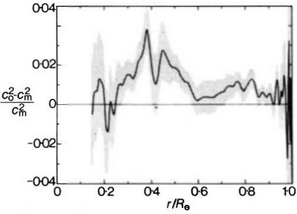
\includegraphics[height=0.45\textheight,keepaspectratio]{dsoundspeedduvall} 

%\end{column}
%\begin{column}{0.4\textwidth}
\captionof{figure}{%Differenza relativa del profilo di $c_s$ (determinata invertendo \eqref{eq:analinversionc}) per frequenze dei modi calcolate con MSS e osservate. La differenza relativa \'e minore del $5\%$.
Da \cite{christensen1985speed}.}
\label{dsoundduvall}
\end{figure}
%\end{column}
%\end{columns}

\end{frame}

\begin{wordonframe}{Intro modi gravo-acustici-risonanza-MSS}

L'eliosismologia nasce all'inizio degli anni '60 quando Leighton e collaboratori osservarono un comportamento periodico nell'atmosfera solare dovuto a modi gravo-acustici, cio\'e onde gravo-acustiche confinate in gusci sferici di diversa profondit\'a che interferiscono costruttuvamente. %La condizione di risonanza radiale, cio\'e che la cavi\'a contenga un numero intero di lunghezze d'onda e tenendo conto di uno sfasamento ai bordi della cavit\'a, permette
Le frequenze osservate compongono la parte ad alte frequenze dello spettro dei modi solari, cio\'e onde acustiche la cui forza di richiamo \'e la perturbazione della pressione, e usando la condizione di risonanza radiale (la cavit\'a contiene un numero intero di lunghezze d'onda e un fattore di fase che tiene conto della riflessione in superficie) \'e possibile ricavare il profilo radiale della velocit\'a del suono all'interno del Sole.

Le piccol differenz nel profilo radiale della velocit\'a del suono ricavato dalle frequenze osservate e quello calcolato tramite un modello solare supporta il modello proposto per spiegare il fenomeno oscillatoria e supporta inoltre il modello solare standard. Descrivo le caratteristiche fondamentali del Sole.


\end{wordonframe}

\part{Modello solare e osservabili sismologiche}\label{part:MSS}
\frame{\partpage}

\begin{frame}{Argomenti}
  \tableofcontents[part=1,hideallsubsections%,pausesections
  ]
  % You might wish to add the option [pausesections]
\end{frame}

\section{Modello solare}

\begin{frame}{Dati osservativi}%<handout:0 beamer:0>

\begin{block}{Et\'a, luminosit\'a, massa, raggio solari}
\begin{tabular}{l|c}
\hline
$\agesun{}$&\SI[separate-uncertainty=true]{4.57\pm0.02e9}{\year}\\
\hline
$\rsun{}$&\SI{695658+-140}{\kilo\meter}\\
\hline
$G\msun$&\num{132712440018+-8}\SI{e9}{\cubic\meter\per\square\second}\\
\hline
$\lsun{}$&\SI{3.8275+-0.0014e33}{\erg\per\second}\\
\hline
\end{tabular}
%\caption[Osservabili solari principali.]{Osservabili solari principali. \cite{haberreiter2008solving}.}
\label{tab:sunO}
\end{block}

\begin{block}{Simmetria sferica}
Deviazioni da forma sferica trascurabili (campi magnetici, rotazione)
\end{block}


\end{frame}

\begin{wordonframe}{Ipotesi e giustificazione struttura equilibrio idrostatico}

La costruzione di un modello solare \'e molto meno incerta rispetto a una stella qualsiasi poich\'e \'e nota la distanza tramite lo studio delle orbite dei corpi celesti attorno al Sole, l'et\'a di formazione del sistema solare tramite studio dei meteoriti, la luminosit\'a, e il raggio tramite la misura delle dimensioni apparenti del disco solare.

Il modello solare s

\end{wordonframe}

\begin{frame}{Dati osservativi}

\begin{block}{Composizione chimica}

%\begin{itemize}[noitemsep,topsep=0pt,parsep=0pt,partopsep=0pt]
Righe di assorbimento della fotosfera.

Meteoriti CI: primordiale (refrattari).

\end{block}


\begin{table}[]

\pgfplotstabletypeset[
every head row/.style={
 before row={\toprule &\multicolumn{4}{c|}{Attuale}
 %&\multicolumn{4}{c|}{Primordiale}
 \\\midrule},
 every last row/.style={after row=\bottomrule},
 after row={\midrule}
},
every nth row={2}{before row=\midrule},every last row/.style={after row=\bottomrule},
every first column/.style={column type/.add={|}{}},
every last column/.style={column type/.add={}{|}},
columns/x/.style = {column type/.add={|}{}},
columns/xi/.style = {column type/.add={|}{}},
display columns/0/.style={column name={}},
display columns/1/.style={column name={$X$}},
display columns/2/.style={column name={$Y$}},
display columns/3/.style={column name={$Z$}},
display columns/4/.style={column name={$\frac{Z}{X}$}},
%display columns/5/.style={column name={$X$}},
%display columns/6/.style={column name={$Y$}},
%display columns/7/.style={column name={$Z$}},
%display columns/8/.style={column name={$\frac{Z}{X}$}},
create on use/authors/.style={create col/set list={
%Anders \& Grevesse (1989),Grevesse \& Noels (1993),
Grevesse et al. (1998),Lodders (2003),Asplund et al. (2005),Lodders et al. (2009),\cite{asplund2009chemical},\cite{caffau2011solar}}},
columns/authors/.style={string type},
columns={authors,x, y, z, zx
%,xi,yi,zi, zxi
},
/pgf/number format/precision=4
     ]{asplund.txt} %%%
\captionof{table}{Metallicit\'a attuale determinata da varii autori.}\label{tab:Zhistory}
\end{table}

\end{frame}


\section{Equilibrio idrostatico e termico}

\begin{frame}{Equilibrio idrostatico}

%\begin{equation*}
%\tau_{idro}^{\odot}= \sqrt{\frac{R^3}{GM}}\approx\frac{1}{2}(G\overline{\rho})\expy{-\frac{1}{2}}\approx\SI{27}{\minute}
%\end{equation*}


\begin{block}{Conservazione momento (Macroscopico)}

\begin{equation*}
\TDy{r}{P}=-\frac{Gm(r)\rho(r)}{r^2}%\label{eq:fidroequilibrio}
\end{equation*}

\end{block}

\begin{block}{Conservazione momento (microscopico)}
\begin{align*}
&\vec{F}_i=-\nabla P_i+n_i(q_i\vec{E}+m_i\vec{g})\\
&=\sum_{i\neq j}\vec{R}_{ij}
\end{align*}

\end{block}

\end{frame}

\begin{frame}{Conservazione energia interna}

\begin{align*}
&\TDy{t}{q}=\epsilon-\frac{1}{\rho}\nabla\cdot\vec{F}\\%\label{eq:heatgl}
&\TDy{r}{L}=4\pi r^2[\rho\epsilon-\rho\TDof{t}u+\frac{P}{\rho}\TDy{t}{\rho}]%\label{eq:fenergyconservation}
\end{align*}


\end{frame}


\section{Meccanismi di trasporto dell'energia}

\begin{frame}{Trasporto radiativo}

\begin{block}{Equilibrio termodinamico locale}
%Il flusso di energia verso la superficie \'e generato da una piccola anisotropia nell'intensit\'a descritta al prim'ordine tramite:
\begin{align*}
%&I_{\nu}=B(\nu,T)-\frac{1}{\kappa_{\nu}'\rho}\nabla_s B(\nu,T)\\
%P_{rad}=\int\,d\nu\frac{4\pi}{3c}B_{\nu}=\frac{1}{3}aT^4\\
%\vec{F}=-\frac{4\pi}{3\kappa\rho}\nabla B=-\frac{4\pi}{3\kappa\rho}\nabla B=-\frac{c}{\kappa\rho}\nabla P_{rad}\\
&\frac{dI_{\nu}}{\rho\,ds}=\kappa_{\nu}B_{\nu}(T)-\kappa_{\nu}I_{\nu}\\
%\frac{1}{\kappa}=(\frac{acT^3}{\pi})\expy{-1}\intzi{}\,d\nu\frac{1}{\kappa_{\nu}}\PDy{T}{B(\nu,T)}\label{eq:rosselandopacity}
&\vec{F}=-\frac{4\pi}{3\kappa\rho}\nabla B(T)=-\frac{c}{\kappa\rho}\nabla P_{rad}
\end{align*}
\end{block}

\begin{block}{Gradiente radiativo}

\begin{equation*}
\nrad{}=\Dcvar{\PDly{P}{T}}{rad}=\frac{3}{16\pi acG}\frac{\kappa l(r)P}{m(r)T^4}%\label{eq:radiativegradient}
\end{equation*}

\end{block}

\end{frame}

\begin{wordonframe}{Trasporto radiativo}

Il trasporto radiativo nell'interno solare \'e descritto considerando il flusso di fotoni  dalle regioni interne pi\'u calde alla superficie come un processo diffusivo e poich\'e il cammino libero medio di un fotone $\invers{\kappa\rho}$ \'e molto piccolo. Posso quindi considerare la radiazione localmente in equilibrio con la materia cio\'e emissione di corpo nero descritta dalla funzione di Plank $B_{\nu}(T)$ (emissivit\'a per unit\'a di frequenza:$B(T)=\frac{ac}{4\pi}T^4$). La soluzione dell'equazione del trasporto radiativo \'e la somma di tutti i contributi $B_{\nu}(-\tau_{\nu})$ pesati dall'esponenziale che descrive l'assorbimento del plasma solare e si pu\'o dimostrare che in condizioni solari il flusso verso la superficie \'e proporzionale a $\nabla B_{\nu}(T)$ (gradiente locale: Espansione $B(\tau_{\nu})$) e al flusso totale integrando sulle frequenze. Infine ricordando che la pressione di radiazione \'e $P_{rad}=\int\,d\nu\frac{4\pi}{3c}B_{\nu}=\frac{1}{3}aT^4$ trovo la relazione tra flusso e gradiente termico.

\end{wordonframe}

\begin{frame}{Trasporto convettivo}

\begin{align*}
&\rho\PtwoDy{t}{(\Delta r)}=-g\Delta\rho=-g[\Dcvar{\TDy{r}{\rho}}{e}-\Dcvar{\TDy{r}{\rho}}{amb}]\Delta r=-N^2\Delta r\\
&N^2=g(\frac{1}{\Gamma_1P}\TDy{r}{P}-\frac{1}{\rho}\TDy{r}{\rho})=g(\frac{1}{\densityscale{}}-\frac{g}{c_s^2})%\label{eq:bvfs}
\end{align*}

\begin{columns}[t]

\begin{column}{0.6\textwidth}

\begin{figure}[!h]
    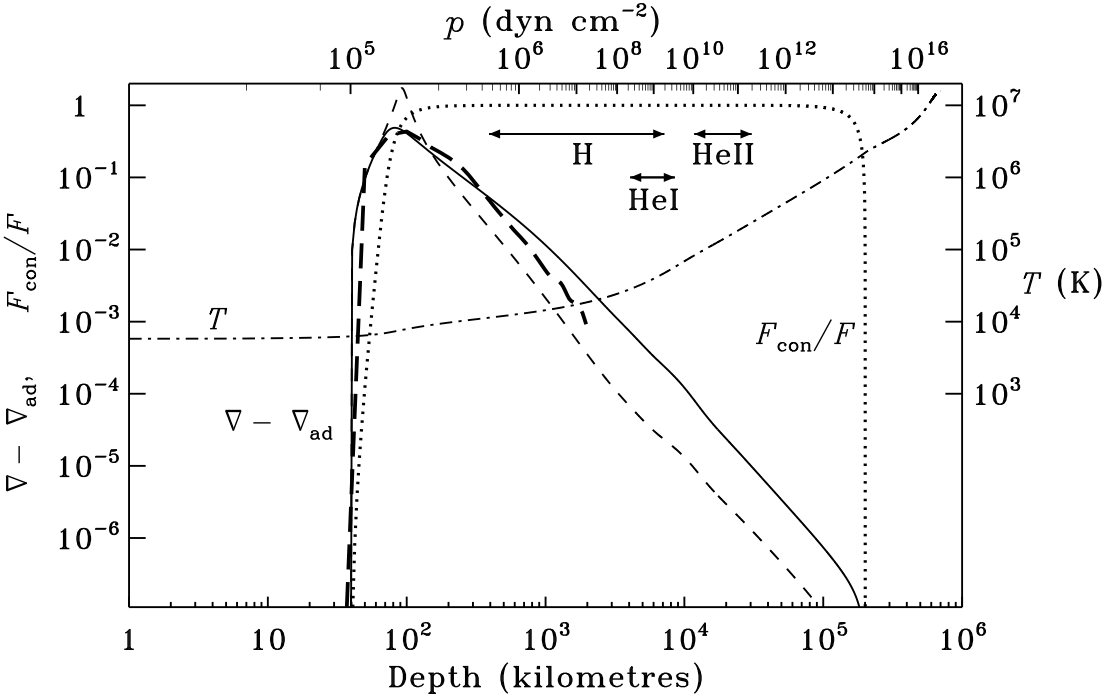
\includegraphics[width=0.95\textwidth,keepaspectratio]{proportionflux}
    \caption{Da \cite{christensen1997effects}.}
    \label{fluxproportion}
\end{figure}

\end{column}

\begin{column}{0.4\textwidth}

\begin{align*}
&F_{con}=\exv{\rho vc_P\Delta T}\\%\label{eq:convectiveflux}
&\nabla-\nad=\nabla-\nabla'+(\nabla_e-\nad{})
\end{align*}


\end{column}

\end{columns}

\end{frame}


\section{Input fisici del MSS}

\begin{frame}{Modello plasma solare}

\begin{block}{Popolazione di stati atomici. EOS e grandezze termodinamiche.}

Interazioni coulombiane:
\begin{align*}
&\frac{1}{r_D^2}=\frac{4\pi e^2}{kT}\sum Z^2\overline{n}_Z=\frac{4\pi e^2}{kT}N_A\sum_{i}(Z_i^2+Z_i)\frac{\rho X_i}{A_i}\\
%&\zeta=\sum_{i}(Z_i^2+Z_i)\frac{\rho X_i}{A_i}\xrightarrow{FD}\sum_{i}(Z_i^2+\frac{F_{\midfrac{1}{2}}'(\psi)}{F_{\midfrac{1}{2}}(\psi)}Z_i)\frac{\rho X_i}{A_i}
\end{align*}

\end{block}

\begin{block}{Interazioni radiazione-materia}
$\nrad{}$
\end{block}

\end{frame}

\begin{wordonframe}{Modellizzazione plasma solare}

L'opacit\'a \'e determinata dai processi di assorbimento e scattering dei fotoni quindi dal numero dalla densit\'a di particelle che danno luogo a un determinato fenomeno di assorbimento o scattering e dalla sezione d'urto per singola particella.

\end{wordonframe}


\begin{frame}{Reazioni nucleari}

\begin{block}{Fusione idrogeno in elio: catena PP}

\end{block}

\end{frame}

\begin{wordonframe}{Importanza reazioni catena PP}

La funzione $\epsilon(T,\rho,X_i)$ descrive la produzione di energia. Nella fase attuale il Sole produce circa il $99\%$ della luminosit\'a tramite la catena PP e circa $1\%$ tramite ciclo CNO

\end{wordonframe}


\section{Costruzione del modello solare}

\begin{frame}{Equazioni della struttura solare}

%Determino la struttura solare integrando numericamente le equazioni fondamentali della struttura stellare
\begin{subequations}\label{subeqn:stellarstructure}
\begin{align}
&\TDy{r}{m}=4\pi r^2\rho\\
&\TDy{r}{P}=-\frac{Gm(r)\rho(r)}{r^2}\\
&\TDy{r}{T}=\nabla\frac{T}{p}\TDy{r}{p}\\
&\TDy{r}{L}=4\pi r^2[\rho(\epsilon-\epsilon_{\nu})-\rho\TDof{t}u+\frac{P}{\rho}\TDy{t}{\rho}]
\end{align}
\begin{equation}
\PDy{t}{n_i}+\frac{1}{r^2}\PDof{r}(r^2n_iv_i)=\Dcvar{\PDy{t}{n_i}}{Nucl}\label{eq:difffusionchange}
\end{equation}
\end{subequations}
%con $v_i$ velocit\'a di diffusione specie i. Ottengo il profilo radiale delle grandezze $\{P,m,T,L,X_i\}$, note la metallicit\'a iniziale Z, l'equazione di stato $P(\rho,T,X_i)$, l'opacit\'a $\kappa(P,T,X_i)$, il rate di produzione di energia nucleare per grammo $\epsilon(P,T,X_i)$.

\begin{block}{Condizionial bordo}
\begin{itemize}
    \item Superficie: $T(r=\rsun{})$, $P(r=\rsun{})$
    \item Centro: $l(r=0)$, $m(r=0)$.
\end{itemize}
\end{block}

\end{frame}

\begin{frame}{Calibrazione modello solare}

\begin{block}{Abbondanze elio iniziale}
Un maggiore peso molecolare medio comporta un maggiore temperatura nel core di fusione
\end{block}

\begin{block}{efficienza convezione}
Mixing length $l_m=H_p\alpha$
\end{block}

\begin{block}{diffusione}

\end{block}

\end{frame}


% SOS
\part{SSM (sos)}
\begin{comment}
\section{Osservabili stellari/demo beamer}
\begin{frame}<1>[label=noinside]{Modello stellare}{Come indagare la fisica interna a una stella?}
\onslide<1->\begin{block}{Osservabili stellari:}
$L$, $M$, $R$, $T_e$, $(\frac{Z}{X})_{ph}$, $g_{ph}$.
\end{block}
\onslide<1->\begin{block}{Informazioni sulla struttura interna?} Condizione di equilibrio idrostatico
\end{block}
%Teorema Vogt-Russel: $X_i(r)$, $M$ \pause equilibrio (idrostatico/termico) determinano struttura stellare .
%\pause
\onslide<1->\begin{block}{Modello stellare: diagramma di \hr{}.}
\end{block}
\onslide<2->\begin{block}{Descrizione fisica interno stellare: parametri aggiuntivi}
Convezione, diffusione e sedimentazione elementi pesanti, equazione di stato, opacit\'a
\end{block}
\onslide<2->\begin{block}{Astrosismologia}
Restringo spazio parametri sistemi stellari lontani
\end{block}
\end{frame}
{ % all template changes are local to this group.
    \setbeamertemplate{navigation symbols}{}
    \begin{frame}[plain]{Diagramma di \hr{}}
        \begin{tikzpicture}[remember picture,overlay]
            \node[at=(current page.center)] {
                %\includegraphics[width=\paperwidth]{yourimage}
            };
        \end{tikzpicture}
     \end{frame}
}
\againframe<2>{noinside}
\begin{frame}{Pulsazioni stellari}{Modi Normali}
\begin{columns}
\begin{column}{0.5\textwidth}  %%<--- here
    \begin{center}
     %\includegraphics[width=0.5\textwidth]{image1}
     \end{center}
\end{column}
\begin{column}{0.5\textwidth}
\onslide<1-> \begin{block}{Stelle pulsanti}
Onde stazionarie: Pulsazione radiale/non radiale: .
\onslide<2-> meccanismo di eccitazione: solar-like pulsator, Cefeidi.
\onslide<3-> Modo fondamentale $\Pi\approx\tau_{dyn}=\sqrt{\frac{R^3}{GM}}\propto\overline{\rho}\expy{-\frac{1}{2}}$.
\onslide<4-> Modi di oscillazione\onslide<5-> - informazioni sull'interno stellare
\onslide<5-> Elio-sismologia: Modi $\Leftrightarrow$ Modelli solari
\onslide<5-> Astero-sismologia: Modi $\Leftrightarrow$ Spazio parametri modello stellare
\end{block}
\end{column}
\end{columns}
\end{frame}

\end{comment}

\section{Osservabili solari}

\begin{frame}{Dati osservativi}

\begin{block}{Et\'a, luminosit\'a, raggio solari}
\begin{tabular}{l|c}
\hline
$\agesun{}$&\SI[separate-uncertainty=true]{4.57\pm0.02e9}{\year}\\
\hline
$\rsun{}$&\SI{695658+-140}{\kilo\meter}\\
\hline
$G\msun$&\num{132712440018+-8}\SI{e9}{\cubic\meter\per\square\second}\\
\hline
$\lsun{}$&\SI{3.8275+-0.0014e33}{\erg\per\second}\\
\hline
\end{tabular}
%\caption[Osservabili solari principali.]{Osservabili solari principali. \cite{haberreiter2008solving}.}
\label{tab:sunO}
\end{block}

\begin{block}{Simmetria sferica}
Deviazioni da forma sferica trascurabili (campi magnetici, rotazione)
\end{block}

\end{frame}

\begin{frame}{Dati osservativi}

\begin{block}{Composizione chimica}
\begin{itemize}[noitemsep,topsep=0pt,parsep=0pt,partopsep=0pt]
\item Righe di assorbimento: attuale (non $Y_{ph}$)
\item Meteoriti CI: primordiale (refrattari)
\end{itemize}

\begin{table}[]

\pgfplotstabletypeset[
every head row/.style={
 before row={\toprule &\multicolumn{4}{c|}{Attuale}
 %&\multicolumn{4}{c|}{Primordiale}
 \\\midrule},
 every last row/.style={after row=\bottomrule},
 after row={\midrule}
},
every nth row={2}{before row=\midrule},every last row/.style={after row=\bottomrule},
every first column/.style={column type/.add={|}{}},
every last column/.style={column type/.add={}{|}},
columns/x/.style = {column type/.add={|}{}},
columns/xi/.style = {column type/.add={|}{}},
display columns/0/.style={column name={}},
display columns/1/.style={column name={$X$}},
display columns/2/.style={column name={$Y$}},
display columns/3/.style={column name={$Z$}},
display columns/4/.style={column name={$\frac{Z}{X}$}},
%display columns/5/.style={column name={$X$}},
%display columns/6/.style={column name={$Y$}},
%display columns/7/.style={column name={$Z$}},
%display columns/8/.style={column name={$\frac{Z}{X}$}},
create on use/authors/.style={create col/set list={
%Anders \& Grevesse (1989),Grevesse \& Noels (1993),
Grevesse et al. (1998),Lodders (2003),Asplund et al. (2005),Lodders et al. (2009),\cite{asplund2009chemical},\cite{caffau2011solar}}},
columns/authors/.style={string type},
columns={authors,x, y, z, zx
%,xi,yi,zi, zxi
},
/pgf/number format/precision=4
     ]{asplund.txt} %%%
\captionof{table}{Metallicit\'a attuale determinata da varii autori.}\label{tab:Zhistory}
\end{table}

\end{block}

\end{frame}


\section{Strutture autogravitanti in equilibrio}

\begin{frame}{Distribuzione di massa - Conservazione di massa e momento - tempo scala dinamico}

\begin{block}{Massa}

%\begin{align}
%&dm=4\pi r^2\rho \,dr-4\pi r^2\rho v\,dt\label{eq:massvar}\\
%\end{align}

\begin{equation}
\PDy{t}{\rho}+\nabla\cdot(\rho\vec{v})=0\label{eq:continuityeq}
\end{equation}

\begin{equation}
dm=4\pi r^2\rho \,dr\label{eq:massaguscio}
\end{equation}

\end{block}

\begin{block}{Momento}
\begin{align}
&\rho\TDy{t}{\vec{v}}=-\nabla P+\rho\vec{f}\label{eq:motion}\\
&\vec{g}=-\PDy{r}{\Phi}=-\frac{Gm(r)}{r^2}\hat{r}
\end{align}
\end{block}

\end{frame}

\begin{frame}{Equilibrio idrostatico: $\ddvec{r}=0$.}

\begin{align*}
\nabla P=\rho \vec{f}\Label{eq:idrosta} \TDy{r}{P}=-\frac{Gm(r)\rho(r)}{r^2}\Label{eq:fidroequilibrio}
\end{align*}


Per giustificare l'ipotesi di equilibrio idrostatico stimo i tempi caratteristici di evoluzione della struttura solare nel caso la forza dovuta alla pressione o la forza di gravit\'a non fossero bilanciate, approssimando il valore caratteristico della derivata di due variabili con il rapporto del loro valore caratteristico.

\begin{equation}
\tau_{ff}\approx\tau_{esp}\approx\tau_{idro}^{\odot}= \sqrt{\frac{R^3}{GM}}\approx\frac{1}{2}(G\overline{\rho})\expy{-\frac{1}{2}}\approx\SI{27}{\minute}
\end{equation}

\end{frame}

\subsection{Equazione di stato $P(\rho,T)$}

\begin{frame}{Gas perfetto ioni-elettroni}


\begin{equation}
P_G=P_I+P_e=\frac{\rho}{\mu}\gasconstant{}T
\end{equation}

\begin{block}{Peso molecolare medio}
massa media in amu per particella libera
\begin{align}
&\mu=\frac{1}{\bar{n}_HX+\bar{n}_{He}Y+\bar{n}_{Z}Z}\label{eq:meanmw}\\
&\bar{n}_i=\frac{1+f_i}{A_i}
\end{align}

\end{block}


\end{frame}

\subsection{Energia interna per unit\'a di massa}

\begin{frame}{Energia interna: traslazioni}

\begin{align}
&u=\frac{1}{\rho}\sum_i\int f^{(0)}(\vec{p}_i)\frac{p^2_i}{2m_i}=\frac{3}{2}\frac{P}{\rho}=\frac{3}{2}\frac{\gasconstant T}{\mu}\\
&E_i=\int_0^Mu\,dm=\frac{3}{2}\int_M\frac{P}{\rho}\,dm\label{eq:traslintenergy}
\end{align}

 $f^{(0)}(\vec{p}_i)$ \'e il numero di particelle della specie i per unit\'a di volume con impulso in $[\vec{p},\vec{p}+d\vec{p}]$

\end{frame}


\subsection{Correzioni alla legge dei gas perfetti}

\begin{frame}{Correzioni alla legge dei gas perfetti}

\begin{itemize}
\item Degenerazione elettronica ($\Delta P\leq2\%$).

\begin{align}
&P_{FD}=[\exp{\psi(\rho,T)+\midfrac{p^2}{2mKT}}+1]\expy{-1}\\
&n_e=\frac{\rho N_A}{\mu_e}=\frac{8\pi}{3h^3m_e}(2m_eKT)\expy{\midfrac{3}{2}}F_{\midfrac{3}{2}}(\psi(\rho,T))\\
%n_e=\intzi{}\frac{8\pi p^2\,dp}{h^3(\exp{\frac{u_k}{KT}-\psi}+1)}\\
&P_e=\frac{1}{3}\intzi{}pn_e\TDy{p}{u_k}\,dp
\end{align}

\item Pressione di radiazione: $P_r=\frac{1}{3}aT^4$.

\item Ionizzazione.

\end{itemize}

\end{frame}

\begin{frame}{Correzioni alla legge dei gas perfetti: Interazioni coulombiane}

\begin{align}
&\frac{1}{r_D^2}=\frac{4\pi e^2}{kT}\sum Z^2\overline{n}_Z=\frac{4\pi e^2}{kT}N_A\zeta\\
&\zeta=\sum_{i}(Z_i^2+Z_i)\frac{\rho X_i}{A_i}\xrightarrow{FD}\sum_{i}(Z_i^2+\frac{F_{\midfrac{3}{2}}'(\psi)}{F_{\midfrac{3}{2}}(\psi)}_i)\frac{\rho X_i}{A_i}
\end{align}

\begin{equation}
u_c=\frac{1}{2}\int\phi(\vec{r})\rho_c(\vec{r})\,d^3r,\ P_c=\frac{1}{3}u_c
\end{equation}

Regioni di ionizzazione parziale di idrogeno ed elio

\end{frame}

\begin{frame}{EOS}

\begin{itemize}
\item Schema chimico (MHD): atomi e molecole, stati eccitati e diversi gradi di ionizzazione

\item Schema fisico (OPAL): nuclei ed elettroni, potenziale Coulombiano, Schr\"oedinger per un problema a molti corpi.
\end{itemize}

\begin{figure}[!ht]
\subfigure[Popolazione dei diversi gradi di ionizzazione per $\cel{He}{4}{}{}$, CNO, $\cel{Ne}{20}{}{}$, $\cel{Fe}{56}{}{}$. Da \cite{basu2008helioseismology}.]{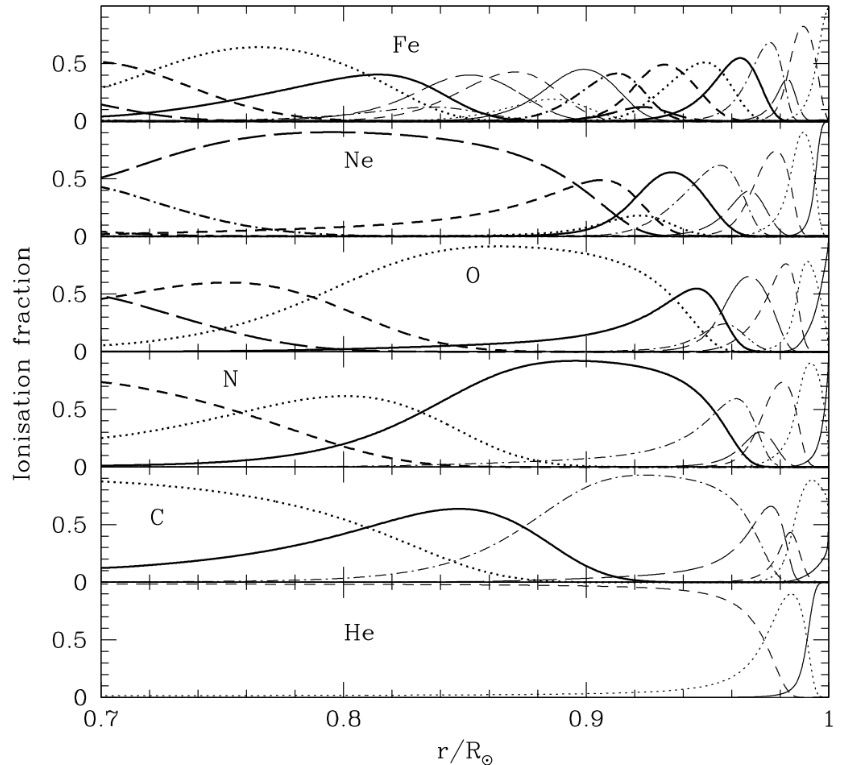
\includegraphics[width=0.4\textwidth,keepaspectratio]{ionfraction}}\label{ionfraction}
%\subcaption{Andamento di $\Gamma_1$ calcolato tramite equazione di stato MHD/OPAL. Da \cite{trampedach2006synoptic}.]{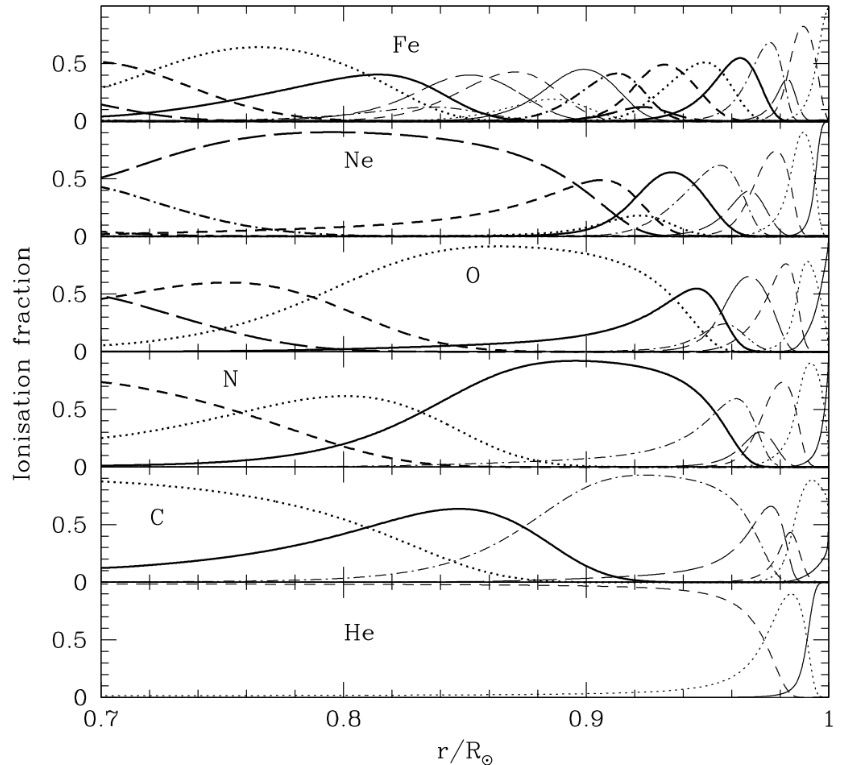
\includegraphics[width=0.4\textwidth,keepaspectratio]{ionfraction}}
~
\subfigure[Confronto $\Gamma_1$ MHD/OPAL. Da \cite{trampedach2006synoptic}.]{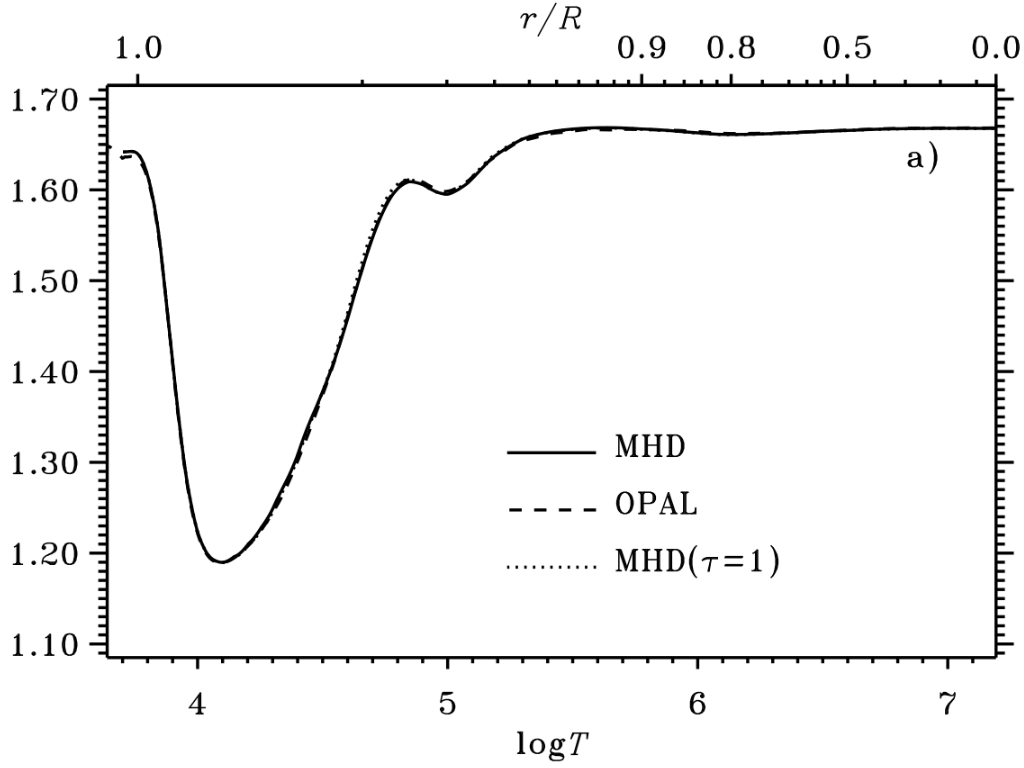
\includegraphics[width=0.4\textwidth,keepaspectratio]{gamma1eos}}
%\subcaption{Profilo radiale della popolazione dei diversi gradi di ionizzazione per $\cel{He}{4}{}{}$, CNO, $\cel{Ne}{20}{}{}$, $\cel{Fe}{56}{}{}$. Stati di ionizzazione maggiore sono pi\'u interni. Da \cite{basu2008helioseismology}.}\label{ionfraction}
%\subcaption{Andamento di $\Gamma_1$ calcolato tramite equazione di stato MHD/OPAL. Da \cite{trampedach2006synoptic}.}\label{fig:gamma1eos}
\end{figure}


\end{frame}


\subsection{Trasporto dell'energia}


\begin{frame}{T Viriale}

Il teorema del viriale esprime una propriet\'a statistica di particelle interagenti: 

L'energia potenziale gravitazionale della stella \'e
\begin{equation}
\Omega=-\int_0^M\frac{Gm(r)}{r}\,dm\label{eq:energiapg}
\end{equation}

\begin{equation}
\frac{1}{2}\TtwoDy{t}{I}=2E_i+\Omega
\end{equation}
con $E_i$ data da \eqref{eq:traslintenergy} e $I=\int r^2\,dm$. In condizioni stazionarie $\frac{1}{2}\TtwoDy{t}{I}\approx0$:
\begin{equation}
0=\int_M\frac{3P}{\rho}\,dm(r)+\Omega
\end{equation}

Detta $W=E_i+\Omega$ l'energia totale della stella, si ha:
\begin{equation}
\Omega=-2E_i\label{eq:virialegpm}
\end{equation}
e dalla conservazione dell'energia $\TDy{t}{W}+L=0$ segue che durante la fase di collasso prima dell'inizio della sequenza principale met\'a dell'energia gravitazionale viene spesa per aumentare l'energia interna e met\'a in luminosit\'a:
\begin{equation}
L=-\frac{1}{2}\dot{\Omega}=\dot{E}_i
\end{equation}

\end{frame}

\begin{frame}{Struttura in equilibrio idrostatico e termico in assenza di reazioni nucleari}

Nel caso in cui la contrazione gravitazionale sia l'unica fonte di energia per una massa gassosa in equilibrio idrostatico, il suo tempo di evoluzione caratteristico \'e il tempo di \kh{}:
\begin{equation}
\tkh{}=\frac{\Omega}{L}\approx\frac{GM^2}{2RL}\approx\SI{1.6e7}{\year}
\end{equation}

cammino libero medio degli atomi e dei fotoni sia breve, si raggiunge rapidamente l'equilibrio idrostatico e termico locale. Il processo di contrazione gravitazionale continua, su tempi-scala termodinamici, fino a che l'energia prodotta dalle reazioni nucleari bilancia l'energia irradiata.


\end{frame}


\subsection{Conservazione dell'energia interna}

\begin{frame}{Prima legge TD}

$dq$ per unit\'a di massa per $dt$:
\begin{align}
&\TDy{t}{q}=\TDy{t}{u}+P\TDof{t}(\frac{1}{\rho})\label{eq:prima}\\
%\TDy{t}{u}+P\TDy{t}{V}
&\TDy{t}{\ln{T}}=\frac{\Gamma_2-1}{\Gamma_2}\TDy{t}{\ln{P}}+\frac{\TDy{t}{q}}{c_PT}\label{eq:primatemp}\\
&\TDy{t}{\ln{P}}=\Gamma_1\TDy{t}{\ln{\rho}}+\frac{\rho(\Gamma_3-1)}{P}\TDy{t}{q}\label{eq:primapres}
\end{align}
Esponenti adiabatici $\Gamma_i$:
\begin{equation}\label{eq:adibatexp}
\Gamma_1=\Dcvar{\TDly{\rho}{P}}{Ad}, \ \Gamma_3-1=\Dcvar{\TDly{\rho}{T}}{Ad},\ \frac{\Gamma_2-1}{\Gamma_2}=\Dcvar{\TDly{P}{T}}{Ad}
\end{equation}

\end{frame}

\subsection{Equilibrio termico}

\begin{frame}{Equilibrio termico}

Scrivo il bilancio di calore per un elemento di massa unitaria di gas:
\begin{equation}
\TDy{t}{q}=\epsilon-\frac{1}{\rho}\nabla\cdot\vec{F}\label{eq:heatgl}
\end{equation}
dove $\epsilon$ \'e l'energia prodotta per unit\'a di tempo e massa e $\vec{F}$ \'e il flusso di energia verso l'esterno generalmente dovuto alla diffusione di fotoni dalla zona pi\'u calda verso la superficie; sostituendo in \eqref{eq:prima} si ha
\begin{equation}
\TDy{r}{L}=4\pi r^2[\rho\epsilon-\rho\TDof{t}u+\frac{P}{\rho}\TDy{t}{\rho}]\label{eq:fenergyconservation}
\end{equation}

Nel caso stazionario:
\begin{equation}
\TDy{t}{q}=0\ \Rightarrow\ dL=4\pi r^2\rho\epsilon\,dr
\end{equation}
e i processi nucleari che avvengono nella parte centrale forniscono il calore per bilanciare il flusso di energia irradiata.

\end{frame}

\subsection{Diffusione}

\begin{frame}{Diffusione elementi}

Velocit\'a di diffusione relativa (\citetitle{aller1960diffusion}):
\begin{equation}
v_{12}=\frac{1}{n_1}\int\,d^3v_1f_1\vec{v}_1-\frac{1}{n_{2}}\int\,d^3v_{2}f_{2}\vec{v}_{2}
\end{equation}

\begin{itemize}\label{itm:diffusionaller}
\item disomogeneit\'a di composizione
\begin{equation}
\propto\frac{1}{c_1c_{2}}\PDy{r}{c_1}
\end{equation}
\item Disomogeneit\'a pressione e forza per unit\'a di massa $F_i$:
\begin{equation}
\frac{m_{2}-m_1}{c_1m_1+c_{2}m_{2}}\frac{1}{P}\PDy{r}{P}-\frac{m_1m_{2}(\vec{F}_1-\vec{F}_{2})}{KT(c_1m_1+c_{2}m_{2})}
\end{equation}
\item disomogeneit\'a temperatura:
\begin{equation}
\frac{K_T}{n_1n_{2}}\frac{1}{T}\PDy{r}{T}
\end{equation}

\end{itemize}

$(-D_{12})/D_{12}=\frac{1}{3}lv_{th}$ con $l\approx(n\sigma)\expy{-1}$ cammino libero medio


\end{frame}

\begin{frame}{Urti}


\begin{equation}
\TDy{t}{f_i}=\PDy{t}{f_i}+\vec{v}_i\cdot\PDy{\vec{r}}{f_i}+\vec{F}_i\cdot\PDy{\vec{v}}{f_i}=-\Div_{\vec{p}}(\vec{s})=C(f_j)\label{eq:Btransport}
\end{equation}
$\tau_{diff}\approx\SI{6e13}{\year}$: soluzione dell'equazione del trasporto di Boltzmann approssimabile con la distribuzione di equilibrio traslata della velocit\'a di diffusione .

Sezione d'urto collisionale di Rutherford:
\begin{align*}
&d\sigma=\frac{4\pi(Z_iZ_j)^2}{\mu^2(\vec{v}-\vec{v}')^4}\frac{d\chi}{\chi^3}\Label{eq:dsruther}L=\int\frac{d\chi}{\chi}=\log{(\frac{1}{\chi_{min}})}\Label{eq:cL}\\
&\lambda=\max{(r_D,a_0)}:\Label{eq:maxb}
\end{align*}

\begin{align*}
\sigma_{ij}\propto \frac{e^4Z_i^2Z_j^2}{(KT)^2}\ln{\Lambda_{st}}\Label{eq:sruther}\ln{\Lambda_{ij}}\propto\ln{[1+0.18769(\frac{4KT\lambda}{Z_iZ_je^2})]}\Label{eq:clog}
\end{align*}

\end{frame}

\begin{frame}{Trasferimento impilso nelle colliioni}

Termine collisionale $C(f)$ (urti con la specie j con distribuzione $f_j$):
\begin{equation}
C(f_i,f_j)=\int\,d^3p_j\,d\sigma|\vec{v}_i-\vec{v}_j|(f_i'f_j'-f_if_j)
\end{equation}

La forza netta dovuta agli urti \'e:
\begin{align}
&\vec{R}_{ij}=\int m\vec{v}C(f_i,f_j)\,d^3v_i%\label{eq:friction}
\vec{R}_{ij}=n_in_j\mu_{ij}\alpha_{ij}\vec{V}_{ij}\label{eq:resistance}\\
&\alpha_{ij}=\frac{\mu_{ij}}{KT}\int v_r^3\sigma^Tf^{(0)}(\vec{v_r})\,d^3v_r%\label{eq:collisionintegral}
\sigma^T=\int(1-\cos{\chi})\,d\sigma\label{eq:sigmatransport}
\end{align}

\begin{block}{Diffusione termica}

La diffusione termica concentra le particelle pi\'u pesanti (e pi\'u cariche) nelle zone pi\'u calde: in presenza di un gradiente termico si ha un trasferimento netto di momento negli urti in direzione del gradiente, in \eqref{eq:friction}, dovuto al maggior numero di particelle energetiche provenienti dalle regioni pi\'u calde, ci\'o \'e dovuto alla dipendenz della sezione d'urto coulombiana dalla velocit\'a relativa $\propto v\expy{-4}$ (probabilit\'a di collisione $\propto v\expy{-3}$).

\end{block}

\end{frame}

\begin{comment}

Considero il problema in cui le due specie hanno velocit\'a relativa media diversa da zero ma piccola rispetto alla velocit\'a termica: nel sistema in cui la prima specie ha velocit\'a media nulla la seconda ha velocit\'a $V_{ij}$ quindi la distribuzione di velocit\'a della prima \'e la distribuzione di equilibrio a temperatura T quella della seconda \'e  la distribuzione di equilibrio a temperatura T traslata di $V_{ij}$, velocit\'a di diffusione:
\begin{equation}
f_j=f_j^{(0)}+\frac{m_j}{KT}(\vec{V}_{ij}\cdot\vec{v}_j)f_j^{(0)}
\end{equation}
da cui si ottiene:
\begin{align}
&\vec{R}_{ij}=n_in_j\mu_{ij}\alpha_{ij}\vec{V}_{ij}\label{eq:resistance}\\
&\alpha_{ij}=\frac{\mu_{ij}}{KT}\int v_r^3\sigma^Tf^{(0)}(\vec{v_r})\,d^3v_r\label{eq:collisionintegral}\\ &\sigma^T=\int(1-\cos{\chi})\,d\sigma\label{eq:sigmatransport}
\end{align}

\end{comment}

\begin{frame}{Sedimentazione gravitazionale}

Nella sedimentazione gravitazionale la forza per unit\'a di volume agente sulle particelle di specie i \'e
\begin{equation}
\vec{F}_i=-\nabla P_i+n_i(q_i\vec{E}+m_i\vec{g})
\end{equation}
e in condizioni di equilibrio il momento trasferito tramite urti con le altre specie \'e uguale alla forza per unit\'a di volume:
\begin{equation}
\vec{F}_i=\sum_{i\neq j}\vec{R}_{ij}%\vec{F}_{ij}=m_{ij}n_in_j\alpha_{ij}\vec{v}_{ij}
\end{equation}


In un plasma costituito da idrogeno, elio ed elettroni per mantenere la neutralit\'a la velocit\'a di diffusione degli elettroni \'e dello stesso ordine di grandezza di quella degli ioni, quindi l'impulso trasferito \'e trascurabile, da cui:
\begin{align}
&F_H\approx F_{HHe}=-\PDy{r}{P_H}+n_H(eE+m_Hg)\\
&F_{He}\approx -F_{HHe}=-\PDy{r}{P_{He}}+n_{He}(2eE+4m_Hg)\\
&E=-\frac{1}{en_e}\PDy{r}{P_e}\\
&v_{HHe}=-\frac{m_{He}T}{m_{HHe}Y\rho \alpha_{HHe}}[\PDy{r}{\ln{(P_eP_H)}}-m_Hg],\ 
n_Hv_H=\frac{(m_{He}n_Hn_{He})}{\rho}v_{HHe}\\
\end{align}

La velocit\'a di diffusione degli elementi pesanti \'e determinata prevalentemente dagli urti con H e He.
Indico con $\eta(A,r)$ la forza per unit\'a di volume sull'elemento di numero atomico Z e di massa A:
\begin{equation}\label{eq:forceperVheavy}
\begin{split}
&\eta(A,r)=-\PDy{r}{P_A}+n_A(Z_Ae\vec{E}+Am_H\vec{g})\\
&=-n_Ak_BT(\PDy{r}{\ln{P_A}}+Z_A\PDy{r}{\ln{P_e}}+\frac{AGm_HM}{r^2k_BT})
\end{split}
\end{equation}

In condizioni stazionarie si ha:
\begin{equation}\label{eq:diffheavystatinary}
\vec{F}_A\approx\vec{R}_{A,H}+\vec{R}_{A,He}=\eta(A,r)
\end{equation}
e poich\'e
\begin{equation}
\frac{\eta(A,r)}{n_Av_H(m_{A,H}n_H\alpha_{A,H})}\propto\frac{1}{XZ_A}
\end{equation}
posso trascurare $\eta(A,r)$ in \eqref{eq:diffheavystatinary} ed esplicitando i contributi $R_{A,H}$ e $R_{A,He}$
ottengo
\begin{equation}\label{eq:diffvelocityA}
v_A(1+2\frac{Y}{X})\approx-v_H
\end{equation}
%&n_Av_A(m_{AH}n_Hw_{AH})(1+2\frac{Y}{X})\approx-n_Av_H(m_{AH}n_Hw_{AH})

\end{frame}

\begin{comment}%%Contributi alla velocit\'a di diffusione di H-He in modello solare. Da \cite{wam88hydrogen}%
\begin{minipage}{\linewidth}
\begin{tikzpicture}
\node[inner sep=0pt] (image) at (0,0)
  {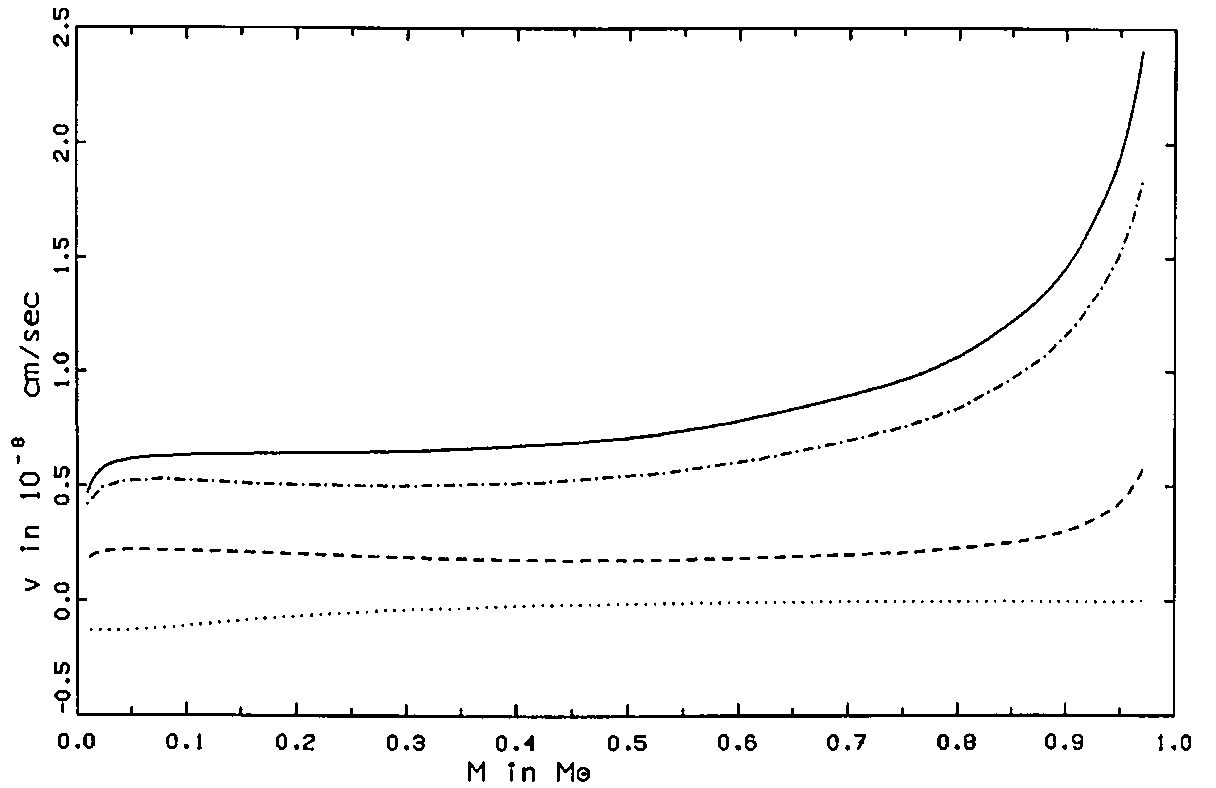
\includegraphics[keepaspectratio=true,width=0.5\textwidth]{Hdiffusion}};
  \draw [thick,dotted] (-3.4,1.5) -- (-3,1.5) node[right] {$\propto\nabla c$};
 \draw [thick,dashed] (-3.4,1.9) -- (-3,1.9) node[right] {$\propto\nabla T$};
    \draw [thick,dash dot] (-3.4,2.3) -- (-3,2.3) node[right] {$\propto\nabla P$};
    \node (caption) at (8.5,-2.5) { \begin{minipage}[c]{0.48\textwidth}
\captionof{figure}{Contributi alla velocit\'a di diffusione di H-He in modello solare. Da \cite{wam88hydrogen}.}%   
    \end{minipage}};
\node[] (massconsdiff) at (8.5,1) {\begin{minipage}[c]{0.48\textwidth}
\end{minipage}
};
\end{tikzpicture}
\end{minipage}
\end{comment}


\section{Trasporto di energia}

\subsection{Trasporto radiativo.}

\begin{frame}{Trasporto radiativo}

$\frac{1}{\kappa\rho}\approx\SI{1}{\cm}$, con $\kappa$ opacit\'a radiativa per unit\'a di massa, quindi considero la radiazione localmente in equilibrio con la materia
%Il flusso di energia verso la superficie \'e generato da una piccola anisotropia nell'intensit\'a descritta al prim'ordine tramite:
\begin{align}
I_{\nu}=B(\nu,T)-\frac{1}{\kappa_{\nu}'\rho}\nabla_s B(\nu,T)\\
P_{rad}=\int\,d\nu\frac{4\pi}{3c}B_{\nu}=\frac{1}{3}aT^4\\
\vec{F}=-\frac{4\pi}{3\kappa\rho}\nabla B=-\frac{4\pi}{3\kappa\rho}\nabla B=-\frac{c}{\kappa\rho}\nabla P_{rad}\\
\nrad{}=\Dcvar{\PDly{P}{T}}{rad}=\frac{3}{16\pi acG}\frac{\kappa l(r)P}{m(r)T^4}\label{eq:radiativegradient}
\end{align}

\end{frame}

\subsection{Opacit\'a.}

\begin{frame}{Opacit\'a media di Rosseland}

\begin{equation}
\frac{1}{\kappa}=(\frac{acT^3}{\pi})\expy{-1}\intzi{}\,d\nu\frac{1}{\kappa_{\nu}}\PDy{T}{B(\nu,T)}\label{eq:rosselandopacity}
\end{equation}

\begin{itemize}[noitemsep,topsep=0pt,parsep=0pt,partopsep=0pt]

\item Scattering fotone-elettrone (sc). Scattering Thomson per $h\nu\ll m_ec^2$ (Scattering Compton per $T\geq\SI{e8}{\kelvin}$)
\begin{align}
&\kappa_{\nu}\propto\frac{r_e^2}{\mu_em_u}, \kappa_{sc}=0.20(1+X)\si{\squared\cm\per\gram}
%&r_e=\SI{2.82e-13}{\cm}
\end{align}


\item Brehmstrahlung inverso (ff).
\begin{equation}
\kappa_{ff}\propto\rho T\expy{-\frac{7}{2}}
\end{equation}
Effetti quantistic: fattore di Gaunt.

\item Reazioni di ionizzazione (bf).
\begin{equation}
\sigma_{bf}=\num{2.82e29}\frac{Z^4}{n^5\nu^3}g(\nu,n,l,Z)\si{\square\cm}
\end{equation}

\item Transizione elettronica a livelli eccitati (bb).

\item Scattering atomici e ione $H^-$. $H^-$:$h\nu>\SI{0.75}{\ev}/\lambda<\SI{1655}{\nano\meter}$.

\end{itemize}

\end{frame}

\begin{frame}{Profilo radiale $\kappa$}

\begin{figure}[!ht]
\centering
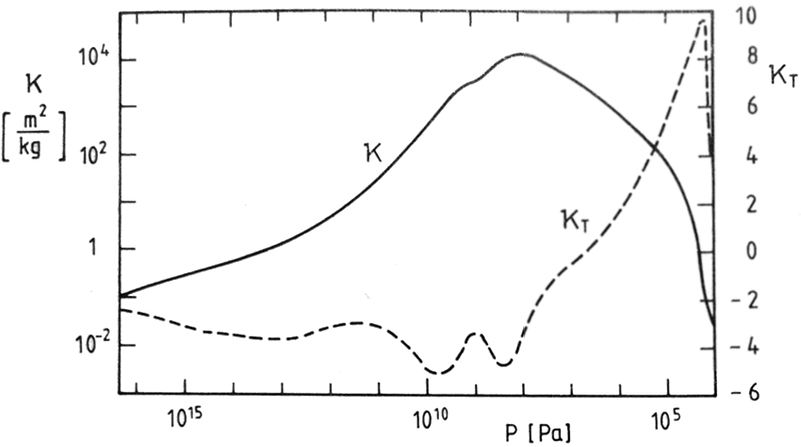
\includegraphics[keepaspectratio,width=0.9\linewidth]{opacitylld}
\caption{Profilo radiale di $\kappa$ e $\PDly{T}{\kappa}$. Da \cite{stix91sun}.}
\end{figure}

\end{frame}

\begin{frame}{Contributi a $\kappa$ per processoper elemento}

\begin{tikzpicture}[]
%([shift={(1.5,0)}]0,0)

\node[anchor=north west] (opint) at (0,0) {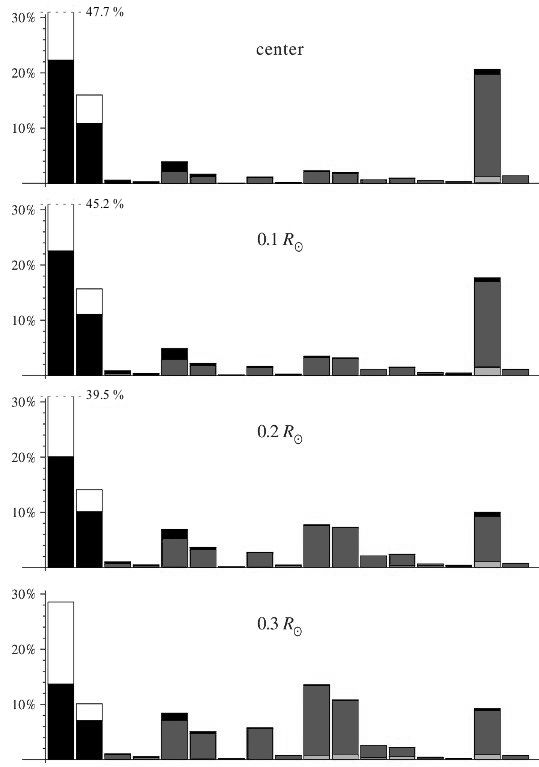
\includegraphics[width=0.45\textwidth,keepaspectratio]{opcontrib-int-g}};
\node[anchor=west,right=2.5cm of opint.east] (opout) {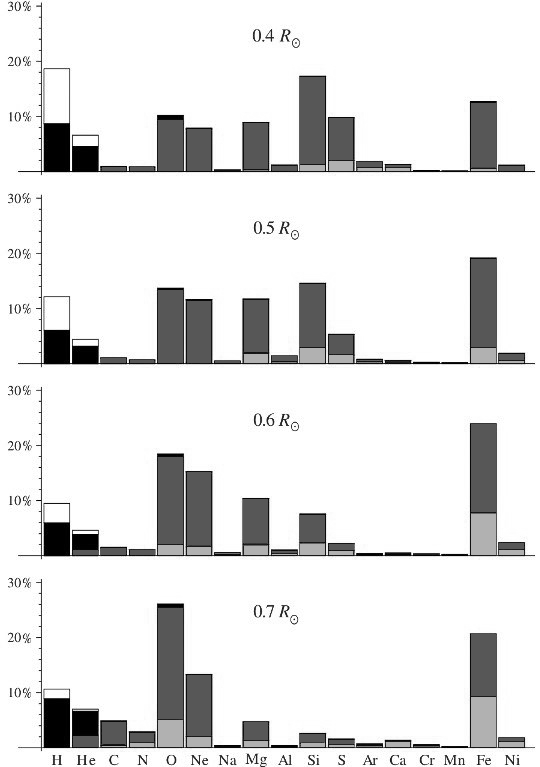
\includegraphics[width=0.45\textwidth,keepaspectratio]{opcontrib-out-g}};
\begin{scope}[scale=0.6]
\node[draw,anchor=west,label={[label distance=2mm]-90:Scattering \Pphoton\Pelectron},minimum size=5mm,below right=1cm and 9mm of opint.east] (sc) {};
\node[draw,label={[label distance=2mm]-90:ff},fill=black,minimum size=5mm,above=10mm of sc] (ff) {};
\node[draw,label={[label distance=2mm]-90:bb},fill=bb,minimum size=5mm,above=10mm of ff] (bb) {};
\node[draw,label={[label distance=2mm]-90:bf},fill=bf,minimum size=5mm,above=10mm of bb] (bf) {};
\end{scope}

\begin{scope}[node distance=2.62mm]
\node[minimum size=2mm,name=hydrogen, right=6.5mm of opint.south west] {\tiny H};
\node[minimum size=2mm,name=helium, right=of hydrogen.west] {\tiny He};
\node[minimum size=2mm,name=carbonium, right=of helium.west] {\tiny C};
\node[minimum size=2mm,name=nitrum, right=of carbonium.west] {\tiny N};
\node[minimum size=2mm,name=oxygen, right=of nitrum.west] {\tiny O};
\node[minimum size=2mm,name=neon, right=of oxygen.west] {\tiny Ne};
\node[minimum size=2mm,name=sodium, right=of neon.west] {\tiny Na};
\node[minimum size=2mm,name=magnesium, right=of sodium.west] {\tiny Mg};
\node[minimum size=2mm,name=alluminium, right=of magnesium.west] {\tiny Al};
\node[minimum size=2mm,name=silicium, right=of alluminium.west] {\tiny Si};
\node[minimum size=2mm,name=sulfur, right=of silicium.west] {\tiny S};
\node[minimum size=2mm,name=argon, right=of sulfur.west] {\tiny Ar};
\node[minimum size=2mm,name=calcium, right=of argon.west] {\tiny Ca};
\node[minimum size=2mm,name=cromum, right=of calcium.west] {\tiny Cr};
\node[minimum size=2mm,name=manganese, right=of cromum.west] {\tiny Mn};
\node[minimum size=2mm,name=ferrum, right=of manganese.west] {\tiny Fe};
\node[minimum size=2mm,name=nikel, right=of ferrum.west] {\tiny Ni};

\end{scope}
 
\node[anchor=north west, below right=1mm and 0.5cm of opint.south west] {\parbox{\textwidth}{\captionof{figure}{Importanza dei varii contributi all'opacit\'a nell'interno solare; composizione GS98. Da \cite{bla11opacity}.}\label{fig:opacitycontrib} }};
 
\end{tikzpicture}

\end{frame}


\subsection{Condizione di in-stabilit\'a dinamica: trasporto convettivo.}

\begin{frame}{Stabilit\'a convettiva}

\begin{equation}
\rho\PtwoDy{t}{(\Delta r)}=-g\Delta\rho=-g[\Dcvar{\TDy{r}{\rho}}{e}-\Dcvar{\TDy{r}{\rho}}{amb}]\Delta r
\end{equation}

\begin{align}
&\frac{d\rho}{\rho}=\alpha\frac{dP}{P}-\delta\frac{dT}{T}+\phi\frac{d\mu}{\mu}\label{eq:deltatherm}
\end{align}

\begin{equation}
\PtwoDy{t}{(\Delta r)}=-g\frac{\delta}{H_P}[\nabla_e-\nabla-\frac{\phi}{\delta}\nmu{}]\Delta r=-N^2\Delta r
\label{eq:galleggiamento}
\end{equation}
\begin{equation}
\nabla_e\approx\nabla_{ad}=\frac{P\delta}{T\rho c_P}
\end{equation}
Vedi STELLAR STRUCTURE  AND EVOLUTION - Mechanical and thermal equilibrium - Equation of state of stellar interiorsPg 32
\begin{equation}
N^2=g(\frac{1}{\Gamma_1P}\TDy{r}{P}-\frac{1}{\rho}\TDy{r}{\rho})=g(\frac{1}{\densityscale{}}-\frac{g}{c_s^2})\label{eq:bvfs}
\end{equation}



\begin{equation}
\nrad{}<\nad+\frac{\phi}{\delta}\nmu{}\label{eq:ledoux}
\end{equation}

\end{frame}

Le stelle con massa $M\leq1.1\msun{}$ hanno una regione radiativa interna mentre la parte esterna \'e convettiva: la regione in cui vale l'uguaglianza in \eqref{eq:ledoux} \'e la base della zona convettiva, la cui posizione \'e determinata dall'aumentare dell'opacit\'a col diminuire della temperatura.
% e dal gradiente adiabatico, il cui valore \'e diminuito dal calore latente di idrogeno ed elio nelle regioni di ionizzazione parziale.

Una maggiore efficienza del trasporto convettivo di energia si riflette in una minore differenza tra il gradiente di temperature adiabatico ed effettivo.

\begin{figure}[!h]
    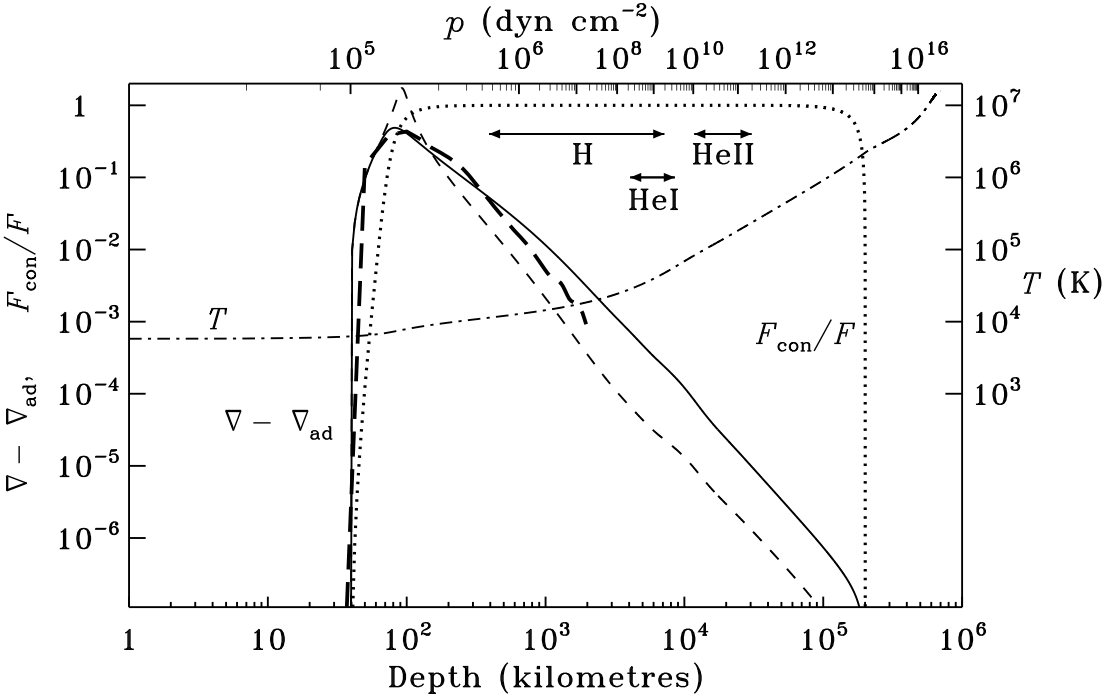
\includegraphics[width=0.9\textwidth,keepaspectratio]{proportionflux}
    \caption{Profilo radiale (profondit\'a in \si{\kilo\meter}) del flusso convettivo $F_c$ rispetto al flusso totale $F$, della super-adiabaticit\'a $\nabla-\nad{}$ e regioni di ionizzazione idrogeno e $\cel{He}{4}{}{}$. Da \cite{gou76convection}.}
    \label{fluxproportion}
\end{figure}

\subsection{Teoria della mixing-length.}

In presenza di convezione il flusso di energia verso l'esterno ha una componente radiativa, determinata dal gradiente di temperatura, e una componente dominante convettiva 
\begin{equation}
F=F_{con}+F_{rad}=\frac{\lsun{}}{4\pi r^2}
\end{equation}
Definisco il gradiente radiativo fittizio:
\begin{equation}
F=\frac{4acG}{3}\frac{T^4m}{\kappa Pr^2}\nrad{}\label{eq:fictionrad}
\end{equation}

Per determinare il gradiente di temperatura effettivo $\nabla$ uso la teoria della mixing-length (\cite{prandtl25tur} e \cite{vitense53kon}):
si considera l'eccesso di calore trasportato dai blob di gas nel moto convettivo $c_P\Delta T$ rispetto all'ambiente, il cui cammino libero medio \'e la mixing-length $l_m=\alpha H_P$, che da luogo al flusso di energia

\begin{equation}
F_{con}=\exv{\rho vc_P\Delta T}\label{eq:convectiveflux}
\end{equation}

dove $\exv{}$ indica una media opportuna sulla sfera di raggio r. Determino il valor medio della differenza di temperatura prendendo come valore caratteristico dello spostamento del blob, considerando moti in entrambi i versi, $\Delta r\approx\frac{l_m}{2}$:
\begin{equation}
\frac{\Delta T}{T}\approx\frac{1}{T}\PDy{r}{(\Delta T)}\frac{l_m}{2}=(\nabla-\nabla_e)\frac{l_m}{2}\frac{1}{H_P}
\end{equation}

Assumo il lavoro medio fatto dalla forza di galleggiamento per unit\'a di massa $-g\frac{\Delta\rho}{\rho}$ uguale al valore medio della forza, cio\'e la met\'a di quello alla superficie sferica data, moltiplicato lo spostamento medio $\frac{l_m}{2}$ quindi, assumendo in oltre che in media met\'a del lavoro fatto dalla forza di galleggiamento sia trasformato in energia cinetica del blob si ottiene

\begin{equation}
v^2=g\delta(\nabla-\nabla_e)\frac{l_m^2}{8H_P}\label{eq:blobvelocity}
\end{equation}

Infine determino gli scambi radiative del blob: il modulo del flusso radiativo \'e proporzionale al gradiente termico in direzione normale alla superficie del blob
\begin{equation}
f=\frac{4acT^3}{3\kappa\rho}|\PDy{n}{T}|
\end{equation}
quindi l'energia scambiata dall'intera superficie S del blob \'e $\lambda=Sf$ che determina, per la prima legge della termodinamica, una variazione di temperatura per unit\'a di tempo:
\begin{equation}
\PDy{t}{T_e}=-\frac{\lambda}{\rho Vc_P}
\end{equation}
indicato con $V$ il volume del blob.

La variazione della temperatura del blob per unit\'a distanza percorsa \'e quindi
\begin{equation}
\Dcvar{\TDy{r}{T}}{e}=\Dcvar{\TDy{r}{T}}{ad}-\frac{\lambda}{\rho Vc_Pv}\label{eq:Tchangelength}
\end{equation}
e approssimando il gradiente normale alla superficie con $\exv{\Delta T}$ ed usando le definizioni \eqref{eq:nablavitense} si ottiene:
\begin{equation}
\frac{\nabla_e-\nad{}}{\nabla-\nabla_e}=\frac{6acT^3}{\kappa\rho^2c_Pl_mv}
\end{equation}

Le 5 equazioni \eqref{eq:fictionrad},\eqref{eq:radiativegradient}, \eqref{eq:convectiveflux}, \eqref{eq:blobvelocity}, \eqref{eq:nablavitense} determinano completamente le variabili $F_{rad}, F_{con}, v, \nabla_e, \nabla$ in funzione di $P,T,l(r),m(r),c_P,\nad{},\nrad{},g$ .



\section{Produzione di energia - reazioni di fusione}

\begin{frame}{Sezione d'urto di fusione}
L'energia liberata dalle reazioni nucleari per grammo per secondo $\epsilon(\rho,T,X_i)$ \'e determinata dalla probabilit\'a che la reazione $X(a,b)Y$ abbia luogo. Sia $E$ l'energia cinetica nel centro di massa dei nuclei, la sezione d'urto $\sigma(E)$ di fusione \'e:
\begin{equation}
\sigma(E)=\pi\lambdabar^2P_0(E)S(E)
\end{equation}

La lunghezza d'onda di de Broglie relativa delle particelle descrive l'indeterminazione sulla posizione nell'urto di due particelle con momento relativo p:
\begin{equation}
\lambdabar=\frac{\hbar}{p}=\frac{\hbar}{\sqrt{2mE}}
\end{equation}

Il fattore astrofisico $S(E)$ descrive l'interazione tra i due reagenti a livello nucleare ed \'e debolmente dipendente dall'energia lontano da risonanze.

La probabilit\'a di attraversamento della barriera coulombiana \'e:
\begin{equation}
P_0(E)=\exp{-2\pi\eta},\ \eta=\sqrt{\frac{m}{2}}\frac{Z_1Z_2e^2}{\hbar E\expy{\frac{1}{2}}}
\end{equation}
Scrivo la sezione d'urto per i nuclei di carica $Z_1$, $Z_2$ e m massa ridotta:
\begin{equation}
\sigma(E)=\frac{S(E)}{E}\exp{-2\pi\eta}\label{eq:fusioncrosssection}
\end{equation}

La funzione $\epsilon(\rho,T,X_i)$ \'e determinata dalla somma di tutti i contributi
\begin{equation}
\epsilon_{ij}=\frac{1}{1+\delta_{ij}}Q_{ij}\frac{\rho N_A^2X_jX_k}{{A_jA_k}}\exv{\sigma v}\label{eq:energyrate}
\end{equation}
dove $Q_{ij}$ \'e l'energia liberata per reazione tra nucleo di specie i e j; $X_i$ indica la frazione in  massa della specie i; $\exv{}$ indica la media sulla distribuzione di Maxwell-Boltzmann
\begin{equation}
f(E)dE\propto\frac{E\expy{\frac{1}{2}}}{(kT)\expy{\frac{3}{2}}}\exp{-\frac{E}{kT}}\,dE\label{eq:MB}
\end{equation}

Per determinare $\exv{\sigma v}$ uso il fatto che l'integrando
\begin{equation}
S(E)\exp{-\frac{E}{kT}-\frac{b}{\sqrt{E}}}\label{eq:reactionrateM}
\end{equation}
ha forma approssimativamente gaussiana il cui massimo $E_G$, energia pi\'u probabile di reazione, e FWHM sono:
\begin{equation}
E_G=\SI{5.665}{\kilo\ev} A\expy{\frac{1}{3}}T_7\expy{\frac{2}{3}},\ \Delta E=4.249W\expy{\frac{1}{6}}T_7\expy{\frac{5}{6}}
\end{equation}
posto $W=Z_j^2Z_k^2A=Z_j^2Z_k^2\frac{A_iA_j}{A_i+A_j}$.

Il rate locale per reazioni non risonanti si scrive approssimativamente come:
\begin{equation}
\exv{\sigma v}=\num{1.3005e-15}[\frac{Z_1Z_2}{AT_6^2}]\expy{\frac{1}{3}}fS_{eff}\exp{-\tau}\si{\cubic\cm\per\second},\ \tau=\frac{3E_G}{kT}\approx\num{42.487}(Z_1^2Z_2^2AT_6\expy{-1})\expy{\frac{1}{3}}
\end{equation}
$S_{eff}$ \'e il risultato dell'espansione dell'integrando per $\invers{\tau}\ll1$ ed estrapolato a $E_G$ a partire dal valore a $E(0)$ determinato dalla fisica nucleare.

\end{frame}

\begin{frame}{Reazioni catena PP}


\setmuskip{\thinmuskip}{0mu}\setmuskip{\medmuskip}{0mu}
\tikzset{->-/.style={decoration={
  markings,
  mark=at position .5 with {\arrow{>}}},postaction={decorate}},
-->/.style={decoration={
  markings,
  mark=at position .8 with {\arrow{>}}},postaction={decorate}},
box/.style={%
%draw,
minimum width=25mm,%
    minimum height=6mm,%
    align=center}
}

\begin{tikzpicture}

\begin{scope}[scale=0.8,transform shape]
\node[box] (pp) at (0,0) {$\Pproton{+}\Pproton{\to}\cel{H}{2}{}{}{+}\Pnue{+}\APelectron$};%%pp
\node[box,right=2cm of pp]  (pep) {$\Pproton{+}\Pproton{+}\Pelectron{\to}\cel{H}{2}{}{}+\Pnue$};%%pep
\coordinate[below=0.3cm of pp] (bpp);
\node[left] at (bpp) {$99.76\%$};
\coordinate[below=0.3cm of pep] (bpep);
\node[right] at (bpep) {$0.24\%$};

\coordinate[] (ttriton) at ($(bpp)!0.5!(bpep)$);
\draw[->-] (pp)--(bpp)--(ttriton);
\draw[->-] (pep)--(bpep)--(ttriton);
\node[box,below=0.3cm of ttriton] (triton) {$\Pproton+\cel{H}{2}{}{}\to\cel{He}{3}{}{}+\Pphoton$};%%triton
\coordinate[below=0.3cm of triton] (btriton);
\draw[-->] (ttriton)--(triton.north);
\draw[->-] (triton.south)--(btriton.north);
\coordinate[left=2.5cm of btriton] (tpp1);
\node[left] at (tpp1) {$83.3\%$};
\coordinate[right=2.0cm of btriton] (tberillium7);
\node[above] at (tberillium7) {$16.7\%$};
\coordinate[right=6.5cm of btriton] (thep);
\node[right] at (thep) {$\num{2e-5}\%$};

\draw[] (btriton)--(tpp1);
\draw[] (btriton)--(tberillium7);
\draw[] (tberillium7)--(thep);
\node[box,below=0.5cm of tpp1,label={[xshift=0.1cm, yshift=-1.5cm]PPI}]  (pp1) {$\cel{He}{3}{}{}+\cel{He}{3}{}{}\to\cel{He}{4}{}{}+2\Pproton$};%%pp1
\node[box,below=0.5cm of tberillium7]  (berillium7) {$\cel{He}{3}{}{}+\cel{He}{4}{}{}\to\cel{Be}{7}{}{}+\Pphoton$};%%berillium7
\node[box,below=0.5cm of thep,label={[xshift=-0.1cm, yshift=-1.5cm]HEP}]  (hep) {$\cel{He}{3}{}{}+\Pproton\to\cel{He}{4}{}{}+\APelectron+\Pnue$};%%hep

\draw[->-] (tpp1)--(pp1.north);
\draw[->-] (tberillium7)--(berillium7.north);
\draw[-->] (thep)--(hep.north);

\coordinate[below=0.3cm of berillium7] (bberillium7);
\coordinate[left=1.5cm of bberillium7] (tlithium7);
\node[left] at (tlithium7) {$99.88\%$};
\coordinate[right=2.0cm of bberillium7] (tboron8);
\node[right] at (tboron8) {$0.12\%$};

\node[box,below=0.5cm of tlithium7]  (li7) {$\cel{Be}{7}{}{}+\Pelectron\to\cel{Li}{7}{}{}+\Pnue$};%%Li7
\node[box,below=0.5cm of li7,label={[xshift=0.1cm, yshift=-1.5cm]PPII}] (pp2) {$\cel{Li}{7}{}{}+\Pproton\to2\cel{He}{4}{}{}$};%% PP2

\node[box,below=0.5cm of tboron8]  (b8) {$\cel{Be}{7}{}{}+\Pproton\to\cel{B}{8}{}{}+\Pphoton$};%%B8
\node[box,below=0.25cm of b8]  (be7) {$\cel{B}{8}{}{}\to\cel{Be}{8}{}{}^*+\APelectron+\Pnue$};%%Be8*
\node[box,below=0.25cm of be7,label={[xshift=0.1cm, yshift=-1.5cm]PPIII}]  (pp3) {$\cel{Be}{8}{}{}^*\to2\cel{He}{4}{}{}$};%%pp3

\draw[->-] (berillium7.south)--(bberillium7);
\draw[] (bberillium7)--(tlithium7);
\draw[] (bberillium7)--(tboron8);

\draw[->-] (tlithium7)--(li7.north);
\draw[->-] (li7.south)--(pp2.north);

\draw[->-] (tboron8.south)--(b8.north);
\draw[->-] (b8.south)--(be7.north);
\draw[->-] (be7.south)--(pp3.north);
\end{scope}

\node[anchor=north west]  at ($(0,0)+(-50mm,-1mm)$) {\parbox{0.5\textwidth}{\captionof{figure}{Reazioni catena PP: terminazioni per temperature caratteristiche del centro solare. Da \cite{adelberger2011solar}.}}};

\end{tikzpicture}

\end{frame}

\begin{frame}{Fattore astrofisico}
\centering
\begin{tikzpicture}[ampersand replacement=\&]

\begin{scope}[scale=0.5,transform shape,every node/.style={scale=0.6}]
\node [matrix,ampersand replacement=\&, matrix of nodes,column sep={60pt,between origins},row
    sep={15pt,between origins}] (s)
  {
Reazione \&  $S(0) (keVb)$ \& \parbox{2cm}{\centering Incertezza su $S(E_G) (\%)$}\\
$p(p,\APelectron\Pnue)d$ \& $(4.01 \pm 0.04)10^{-22}$ \& $\pm 0.7$\\
$d(p,\Pphoton)\cel{He}{3}{}{}$ \& ${2.14}10^{-4}\substack{+0.17 \\ -0.16}$ \& $\pm 7.1$\\
$\cel{He}{3}{}{}(\cel{He}{3}{}{},2p)\cel{He}{4}{}{}$ \& $(5.21 \pm 0.27)10^{-3}$ \& $\pm 4.3$\\
$\cel{He}{3}{}{}(\cel{He}{4}{}{},\Pphoton)\cel{Be}{7}{}{}$ \& $0.56 \pm 0.03$ \& $\pm 5.1$\\
$\cel{He}{3}{}{}(p,\APelectron\Pnue)\cel{He}{4}{}{}$ \& $(8.6 \pm 2.6)10^{-20}$ \& $\pm 30$\\
$\cel{Be}{7}{}{}(\Pelectron,\Pnue)\cel{Li}{7}{}{}{\ }^{I}$ \& $ $ \& $\pm 2.0$\\
$p(p\Pelectron,\Pnue)d{\ }^{II}$\& $ $ \& $\pm 1.0$\\
$\cel{Be}{7}{}{}(p,\Pphoton)\cel{B}{8}{}{}$\& $(2.08 \pm 0.16)10^{-2}$ \& $\pm 7.5$\\
%14N(p,7)150 XI.A 1.66 \pm 0.12 (-3.3 \pm 0.2) x 10-3 b (4.4 \pm 0.3) x 10-5 a \pm 7.2
  };
\draw[]({$(s-1-1)!.5!(s-1-2)$} |- s.north) -- ({$(s-1-1)!.5!(s-1-2)$} |- s.south);
\draw[]({$(s-1-2)!.5!(s-1-3)$} |- s.north) -- ({$(s-1-2)!.5!(s-1-3)$} |- s.south);
\node[fit=(s-1-1.south) (s-1-2.south) (s-1-3.south),inner sep=0pt] (R2) {};
\draw[] (R2.south -| s.west) -- (R2.south -| s.east);
 \end{scope}
 
\node (pep) at ($(s.south)+(47mm,-6mm)$) {\parbox{\textwidth}{\begin{equation*}\scriptscriptstyle II: R(p\Pelectron p)=\scriptscriptstyle1.102(1\pm0.01)10^{-4}\midfrac{\rho}{\mu_e}T_6\expy{-1/2}
\scriptscriptstyle[1+0.002(T_6-16)]R(pp)\end{equation*}}};
\node[below=0.1mm of pep] (ec) {\parbox{\textwidth}{\begin{equation*}\scriptscriptstyle I: R(\cel{Be}{7}{}{}(\Pelectron,\Pnue)\cel{Li}{7}{}{})=\scriptscriptstyle5.6(1\pm0.02)10^{-9}\midfrac{\rho}{\mu_e}T_6\expy{-1/2}\scriptscriptstyle[1+0.004(T_6-16)]\si{\per\second}\end{equation*}}};
 
\node[below=0.1mm of ec] (captions) {\parbox{\textwidth}{\captionof{figure}{Fattore astrofisico reazioni catena PP}}};

\end{tikzpicture}

\end{frame}

\begin{frame}{Schermaggio elettronico}

\begin{figure}[!ht]
       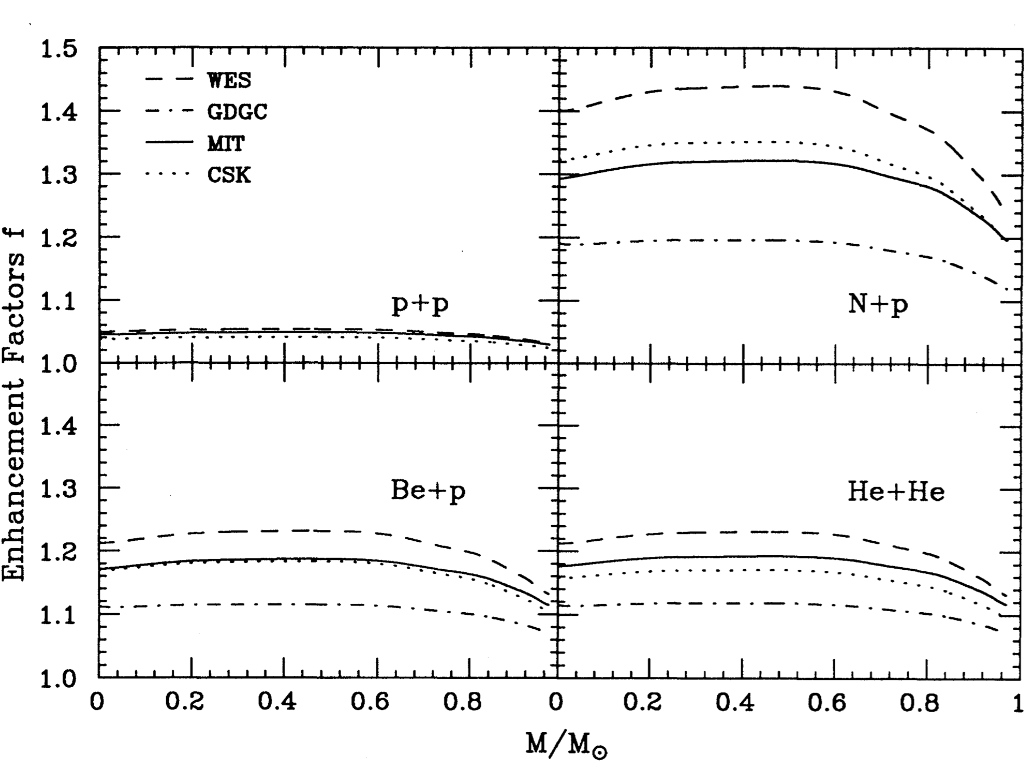
\includegraphics[width=0.4\textwidth,keepaspectratio]{Rscreening}
       \caption{Andamento della correzione di schermaggio degli elettroni secondo diversi schemi. Da \cite{ricci1995screening}.}
\end{figure}

L'energia potenziale dovuta all'interazione di due nuclei $Z_1$ e $Z_2$ a distanza r contiene un contributo delle altre cariche presenti nel plasma:
\begin{equation}
U=\frac{Z_1Z_2e^2}{r}+U_s(r_{12})
\end{equation}
dove il primo termine \'e l'energia potenziale non schermata e il termine $U_s(r_{12})$ il contributo della nuvola elettronica. L'effetto di $U_s$ \'e di aumentare la probabilit\'a di attraversamento della barriera coulombiana. Correggo quindi \eqref{eq:fusioncrosssection} con il fattore moltiplicativo:
\begin{equation}
f=\exp{-\midfrac{U_0}{KT}}\label{eq:screeningfactor}
\end{equation}
dove $U_0=U_s(0)$ poich\'e $r\ll r_D$ e considerando solo la correzione al fattore di penetrazione ($E_G\gg U_0$).

Per determinare $U_0$ considero l'energia potenziale di $Z_1$ e $Z_2$ a distanza $r$
\begin{equation}
U=Z_2e\int_{\infty}^r\PDy{r_1}{\phi_1}\,dr_1=\frac{Z_1Z_2e^2\exp{-\midfrac{r}{r_D}}}{r}
\end{equation}
con $\phi_1$ dato da \eqref{eq:screenedpotential}, e quindi
\begin{equation}
U_s=U-\frac{Z_1Z_2e^2}{r}
\end{equation}

\end{frame}

\begin{frame}{Tempo in sequenza principale}

Sulla base dell'efficienza delle reazioni nucleari, del profilo di densit\'a e temperatura ricavati da un modello solare le terminazione della catena pp $\cel{He}{3}{}{}-\cel{He}{3}{}{}$ e $\cel{He}{3}{}{}-\cel{He}{4}{}{}$ generano rispettivamente $83.3\%$, $16.7\%$ della luminosit\'a totale mentre il ciclo CNO circa $1\%$.

Il tempo trascorso da una stella di massa solare in sequenza principale considerando \'e il tempo necessario per la massa di idrogeno nel core di fusione (le temperature necessarie perch\'e il rate di reazione sia apprezzabile si raggiungono nella regione pi\'u interna che costituisce una frazione $f$ pari al $15\%$ della massa solare) ad esaurirsi:

\begin{equation}
\tau_n\approx\frac{E_n}{L}=\frac{fX\msun Q}{\lsun}\approx\SI{e+10}{\year},\ Q\approx\SI{6.3e18}{\erg\per\gram}
\end{equation}

\end{frame}

\section{Modello solare standard e osservabili sismologiche}




\part{Oscillazioni della fotosfera con grande coerenza spaziale e temporale - Modi normali di cavit\'a risonanti dell'interno solare}\label{part:oscillations}

\frame{\partpage}

\begin{frame}{Argomenti}
  \tableofcontents[part=2,hideallsubsections%,pausesections
  ]
  % You might wish to add the option [pausesections]
\end{frame}

\section{Modi normali della struttura solare}

\begin{frame}{Modi normali: perturbazioni di una struttura a simmetria sferica}
\begin{block}{Equazione del moto perturbato linearizzata}
\begin{equation*}
\rho_0\TDof{t}\vec{v}=\rho_0\PtwoDy{t}{\vec{\xi}}=-\nabla P'+\rho_0\vec{g}'+\rho'\vec{g}_0%\label{eq:emper}
\end{equation*}
\end{block}
\begin{block}{Equazione di continuit\'a e del moto perturbate}
\begin{equation*}
\rho'+\div{(\rho_0\Lvar{\vec{r}})}=0%\label{eq:contper}
\end{equation*}
\end{block}
\begin{block}{Condizione di moto adiabatico}
\begin{equation*}
P'+\vec{\xi}\cdot\nabla P_0=\frac{\Gamma_{1,0}P_0}{\rho}(\rho'+\vec{\xi}\cdot\nabla\rho_0)%\label{eq:adper}
\end{equation*}
\end{block}
\end{frame}

\begin{frame}{Modi normali struttura sferica}

\begin{block}{Onde stazionarie}
\begin{align*}
&Y_{lm}(\theta,\phi)=(-)^mc_{lm}P_l^m(\cos{\theta})\exp{im\phi}\\
&(\rho',P',\Phi')=\exp{i\omega t}[\rho'(r),P'(r),\Phi'(r)]Y_l^m\\
&\vec{\xi}=\exp{i\omega t}(\xi_r(r),\xi_h(r)\PDof{\theta},\frac{\xi_h(r)}{\sin{\theta}}\PDof{\phi})Y_l^m(\theta,\phi)
\end{align*}
\end{block}

\begin{block}{Componente tangenziale dello spostamento perturbato}

\begin{equation*}
\xi_h(r)=\frac{L}{r\omega^2}(\frac{P'(r)}{\rho_0}+\Phi'(r))
\end{equation*}

\end{block}

\end{frame}


\begin{frame}{Modi normali: equazione fondamentale}

\begin{block}{Modi normali}

\begin{subequations}%\label{eigenomega}
\begin{align*}
&\frac{1}{r^2}\TDof{r}(r^2\xi_r)-\frac{\xi_rg}{c^2}+\frac{1}{\rho_0}(\frac{1}{c^2}-\frac{l(l+1)}{r^2\omega^2})P'-\frac{l(l+1)}{r^2\omega^2}\Phi'=0\\
&\frac{1}{\rho_0}(\TDof{r}+\frac{g}{c^2})P'-(\omega^2-N^2)\xi_r+\TDy{r}{\Phi'}=0\\
&\frac{1}{r^2}\TDof{r}(r^2\TDy{r}{\Phi'})-\frac{l(l+1)}{r^2}\Phi'-\frac{4\pi G\rho_0}{g}N^2\xi_r-\frac{4\pi G}{c^2}P'=0
\end{align*}
\end{subequations}

Condizioni al contorno:

Soluzioni regolari per $r=0$: $P'=0$, $\Phi'=0$.

La condizione di non propagazione oltre la fotosfera: $\Lvar{P}=P'+\xi_r\TDy{r}{P}=0$.

\end{block}

\end{frame}

\begin{wordonframe}{Spettro dei modi: frequenze discrete}

Questo \'e il sistema che determina i modi normali: ha soluzioni per $\omega_{nlm}$ discrete. Le condizioni al bordo richiedono regolarit\'a delle perturbazioni in 0 e riflessione totale delle perturbazioni alla superficie solare. $(l,m)$ caratterizzano la dipendenza angolare dei modi mentre n \'e l'ordine radiale che identifica il numero di zeri radiali del vettore spostamento.

L'approssimazione di Cowling, valida per grandi l o n, consiste nel trascurare la perturbazione al potenziale gravitazionale, restringendosi quindi alle prime 2 equazioni.

\end{wordonframe}

\begin{frame}{Spettro dei modi solari}

\begin{figure}[!ht]



%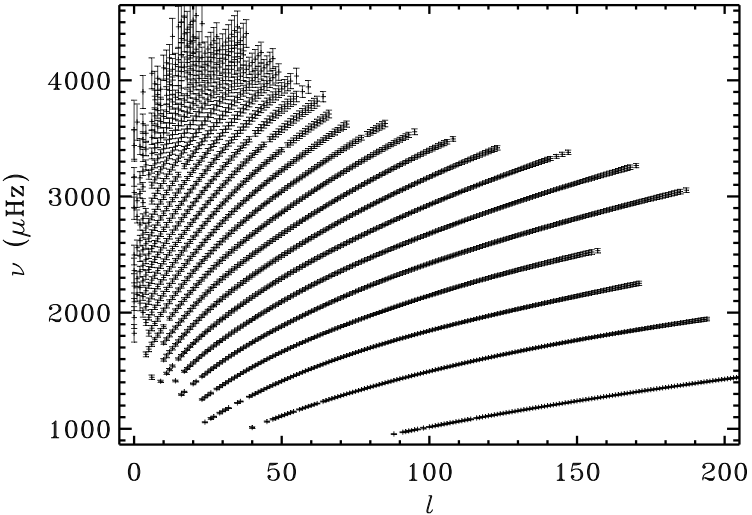
\includegraphics[keepaspectratio,width=0.95\textwidth]{midlmodes}
%\caption{I picchi della densit\'a spettrale si dispongono su creste in cui \'e concentrata la potenza in accordo al modello. Determinata usando i primi 144 giorni di osservazione di MDI con $l\leq300$. Da \cite{chr02helioseismology}.}\label{fig:midlmodes}

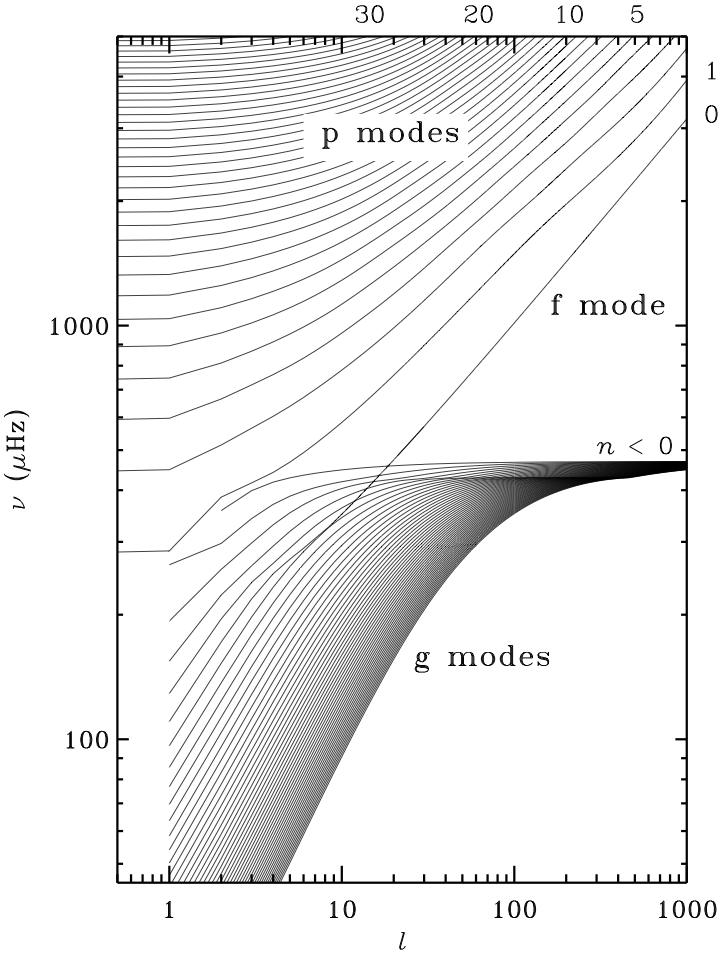
\includegraphics[keepaspectratio,height=0.85\textheight]{nrmodesLAWE}
\caption{Modi adiabatici calcolati sulla base di un modello solare. Da \cite{chr02helioseismology}.}\label{fig:nrmodesLAWE}

\end{figure}

\end{frame}

\begin{wordonframe}{Spettro dei modi: modi p, modi g, modi f}

La figura mostra le frequenze per cui il sistema dei modi ha soluzione. Le frequenze sono discrete distribuite sulle linee in figura rappresentanti soluzioni con stesso ordine radiale n.


\end{wordonframe}

\begin{frame}{Cavit\'a risonanti}



\begin{figure}[!ht]
\centering
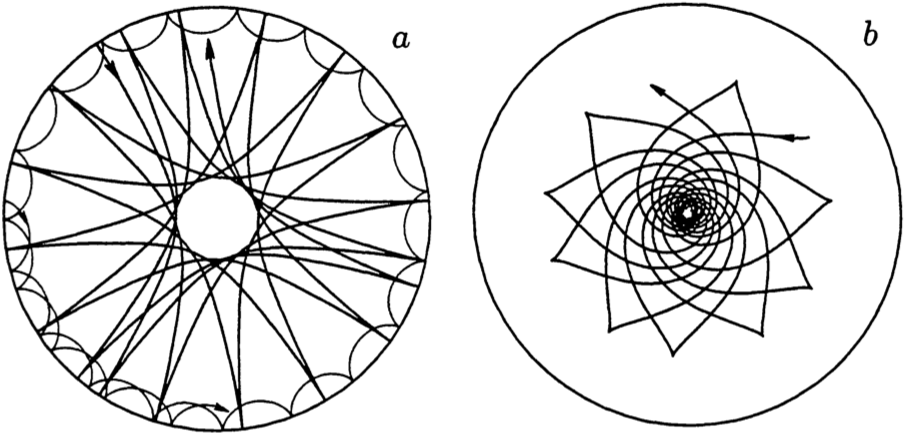
\includegraphics[keepaspectratio,width=0.6\textwidth]{raypath-gp}
\caption{Da\cite{gou91seismic}.}
\end{figure}
%$\omega_c=\frac{c_s}{2\densityscale{}}\sqrt{1-2\TDy{r}{\densityscale{}}}\propto T\expy{-\frac{1}{2}}$
%$S_l^2=\frac{l(l+1)c_s^2}{r^2}$.
%$N^2=g(\frac{1}{\Gamma_1P}\TDy{r}{P}-\frac{1}{\rho}\TDy{r}{\rho})=g(\frac{1}{\densityscale{}}-\frac{g}{c_s^2})$
\begin{align*}
&\omega_A=\frac{c_s}{2\densityscale{}}\sqrt{1-2\TDy{r}{\densityscale{}}}\propto T\expy{-\frac{1}{2}}\\%\label{eq:acusticcutoff} \intxt{quindi ottengo la relazione di dispersione:}
&k_r^2=\frac{\omega^2-\omega_A^2}{c^2}+S_l\frac{N^2-\omega^2}{c^2\omega^2}\\%\label{eq:localdispersion}\intxt{dove ho definito le frequenze critiche per i modi gravo-acustici}
&\omega\int_{r_1}^{r_2}\sqrt{1-\frac{\omega_A^2}{\omega^2}-\frac{S_l^2}{\omega^2}(1-\frac{N^2}{\omega^2})}\,\frac{dr}{c}\approx\pi(n-\frac{1}{2})%\label{eq:JWKBmode}
\end{align*}

\end{frame}

\begin{frame}{Osservazione campo di velocit\'a solare}

\begin{figure}[!ht]



%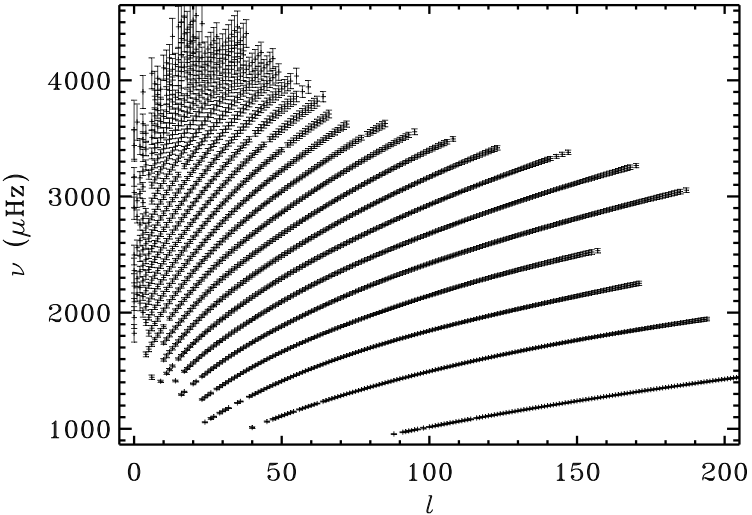
\includegraphics[keepaspectratio,width=0.95\textwidth]{midlmodes}
%\caption{I picchi della densit\'a spettrale si dispongono su creste in cui \'e concentrata la potenza in accordo al modello. Determinata usando i primi 144 giorni di osservazione di MDI con $l\leq300$. Da \cite{chr02helioseismology}.}\label{fig:midlmodes}

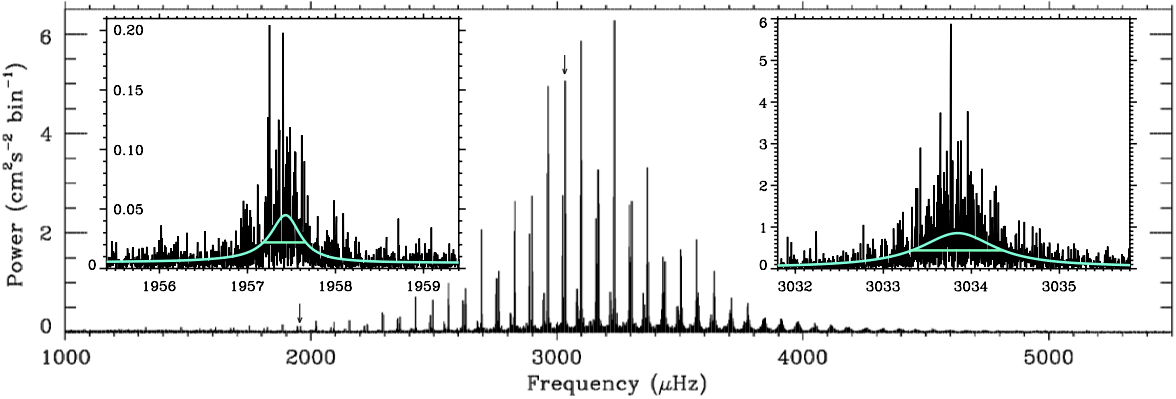
\includegraphics[keepaspectratio,width=0.95\textwidth]{PSD}
\caption{Da \cite{houdek2006stochastic}.}\label{fig:PSD}

\end{figure}

\end{frame}

%%% SOS
\part{OSCILLAZIONI SOS}
\subsection{Osservabili stellari}

\begin{frame}<1>[label=noinside]{Modello stellare}{Come indagare la fisica interna a una stella?}

\onslide<1->\begin{block}{Osservabili stellari:}
$L$, $M$, $R$, $T_e$, $(\frac{Z}{X})_{ph}$, $g_{ph}$.
\end{block}

\onslide<1->\begin{block}{Informazioni sulla struttura interna?} Condizione di equilibrio idrostatico
\end{block}

%Teorema Vogt-Russel: $X_i(r)$, $M$ \pause equilibrio (idrostatico/termico) determinano struttura stellare .
%\pause

\onslide<1->\begin{block}{Modello stellare: diagramma di \hr{}.}
\end{block}

\onslide<2->\begin{block}{Descrizione fisica interno stellare: parametri aggiuntivi}
Convezione, diffusione e sedimentazione elementi pesanti, equazione di stato, opacit\'a
\end{block}

\onslide<2->\begin{block}{Astrosismologia}
Restringo spazio parametri sistemi stellari lontani
\end{block}

\end{frame}


{ % all template changes are local to this group.
    \setbeamertemplate{navigation symbols}{}
    \begin{frame}[plain]{Diagramma di \hr{}}
        \begin{tikzpicture}[remember picture,overlay]
            \node[at=(current page.center)] {
                %\includegraphics[width=\paperwidth]{yourimage}
            };
        \end{tikzpicture}
     \end{frame}
}



\againframe<2>{noinside}


\section{Osservazioni}

\subsection{Fitting polinomiale: inversione ''1.5-D''.}

\begin{frame}<1>[label=noinside]{Modello stellare}{Come indagare la fisica interna a una stella?}



\onslide<1->\begin{block}{Rotazione superficiale}
\begin{equation*}
\frac{\Omega(\theta)}{2\pi}=\SI{451.5}{\nano\hertz}-\SI{65.3}{\nano\hertz}\cos^2{\theta}-\SI{66.7}{\nano\hertz}\cos^4{\theta}
\end{equation*}

\end{block}

\onslide<1->\begin{block}{Informazioni sulla struttura interna?} Condizione di equilibrio idrostatico
\end{block}

%Teorema Vogt-Russel: $X_i(r)$, $M$ \pause equilibrio (idrostatico/termico) determinano struttura stellare .
%\pause

\onslide<1->\begin{block}{Modello stellare: diagramma di \hr{}.}
\end{block}

\onslide<2->\begin{block}{Descrizione fisica interno stellare: parametri aggiuntivi}
Convezione, diffusione e sedimentazione elementi pesanti, equazione di stato, opacit\'a
\end{block}

\onslide<2->\begin{block}{Astrosismologia}
Restringo spazio parametri sistemi stellari lontani
\end{block}

\end{frame}


\subsection{Osservazione dello splitting in m: inversione ''2D''.}

\begin{figure}[!ht]
\centering
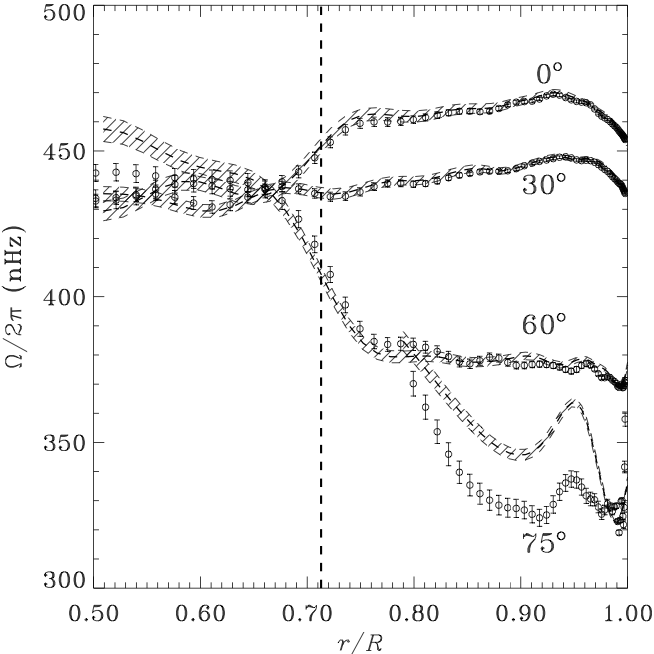
\includegraphics[keepaspectratio,width=0.8\textwidth]{invertedrotation}
\caption{Inversione della velocit\'a di rotazione a diverse latitudini. La linea verticale tratteggiata indica la base della zona convettiva. Da \cite{chr02helioseismology}.}
\end{figure}

Considero la correzione al primo ordine in $\Omega$. Il campo di velocit\'a rotazionale in coordinate sferiche \'e 
\begin{align}
&\vec{v_0}=(0,0,r\Omega\sin{\theta})=\vecp{\Omega}{r}\\
&\vec{\Omega(r,\theta)}=(\Omega(r,\theta)\cos{\theta},-\Omega(r,\theta)\sin{\theta},0)
\end{align}

In assenza di moti macroscopici il termine d'inerzia \'e $\rho_0\TDy{t}{\vec{v}}=\rho_0\PtwoDy{t}{\vec{\xi}}$, mentre in caso di rotazione si ha
\begin{equation}
\rho_0(\PDof{t}+\scap{v_0}{\nabla})^2\vec{\xi}
\end{equation}

Considero il termine dovuto alla rotazione come una piccola correzione alle frequenze dei modi
\begin{align}
&\omega_{(l,m)}+\Delta\omega_{(l,m)}&\intertext{quindi l'equazione del moto al primo ordine nella perturbazione, con $\alpha=(l,m)$, \'e}\nonumber\\
&\rho_0(\omega_{\alpha}^2+2\omega_{\alpha}\Delta\omega_{\alpha})\vec{\xi}=\nabla P_1-\frac{\rho_1}{\rho_0}\nabla P_0+\rho_0\nabla\Phi_1+2i\omega_{\alpha}\rho_0(\scap{v_0}{\nabla})\vec{\xi}\\
&\intertext{da cui si deduce}\nonumber\\
&\Delta\omega_{\alpha}=\frac{i\int\rho_0\xi_{\alpha}^*(\scap{v_0}{\nabla})\xi_{\alpha}}{\int\rho_0\xi_{\alpha}^*\xi_{\alpha}}=\frac{-m\int\rho_0\Omega\xi_{\alpha}^*\xi_{\alpha}\,dV+i\int\rho_0\xi_{\alpha}^*(\vecp{\Omega}{\xi_{\alpha}})\,dV}{\int\rho_0\xi_{\alpha}^*\xi_{\alpha}}
\end{align}

Il problema di trovare $\Omega(r,\theta)$ dalla differenza $\Delta\omega_{\alpha}$ \'e lineare in $\Omega$ quindi $\Delta\omega_{\alpha}\propto\Omega$. Per determinare quindi la rotazione dobbiamo conoscere l'autovalore $\xi_{\alpha}$ dello stato imperturbato.

%Per rotazione puramente radiale $\Omega(r)$ la relazione tra lo splitting delle frequenze e la rotazione \'e
%\begin{equation}
%\Delta\omega_{\alpha}=-m\frac{\int_0^{\rsun{}}\rho_0\Omega\{|\xi_r-\xi_h|^2+[l(l+1)-2]|\xi_h|^2\}r^2\,dr}{\int_0^{\rsun{}}\rho_0\{|\xi_r|^2+l(l+1)|\xi_h|^2\}r^2\,dr}=\int_0^{\rsun{}}K_{\alpha}(r)\Omega(r)\,dr
%\end{equation}
%Any given $\Delta\omega_{\alpha}$ samples angular velocity in the depth range corresponding to $\xi_{\alpha}$.

La velocit\'a angolare contribuisce a $\Delta\omega_{\alpha}$ negli strati in cui $\xi_{\alpha}$ \'e apprezzabile. Nel caso di rotazione dipendente solo da r si ha che $\Delta\omega_{\alpha}$ \'e lineare in m: ho $2l+1$ frequenze equispaziate.



\part{Tecniche e risultati di inversione}\label{part:inverseproblem}

\frame{\partpage}

\begin{frame}{Argomenti}
  \tableofcontents[part=3,hideallsubsections%,pausesections
  ]
  % You might wish to add the option [pausesections]
\end{frame}

\part{INVERSIONE SOS}

\section{Osservabili stellari/demo beamer}

\begin{frame}<1>[label=noinside]{Modello stellare}{Come indagare la fisica interna a una stella?}

\onslide<1->\begin{block}{Osservabili stellari:}
$L$, $M$, $R$, $T_e$, $(\frac{Z}{X})_{ph}$, $g_{ph}$.
\end{block}

\onslide<1->\begin{block}{Informazioni sulla struttura interna?} Condizione di equilibrio idrostatico
\end{block}

%Teorema Vogt-Russel: $X_i(r)$, $M$ \pause equilibrio (idrostatico/termico) determinano struttura stellare .
%\pause

\onslide<1->\begin{block}{Modello stellare: diagramma di \hr{}.}
\end{block}

\onslide<2->\begin{block}{Descrizione fisica interno stellare: parametri aggiuntivi}
Convezione, diffusione e sedimentazione elementi pesanti, equazione di stato, opacit\'a
\end{block}

\onslide<2->\begin{block}{Astrosismologia}
Restringo spazio parametri sistemi stellari lontani
\end{block}

\end{frame}

{ % all template changes are local to this group.
    \setbeamertemplate{navigation symbols}{}
    \begin{frame}[plain]{Diagramma di \hr{}}
        \begin{tikzpicture}[remember picture,overlay]
            \node[at=(current page.center)] {
                %\includegraphics[width=\paperwidth]{yourimage}
            };
        \end{tikzpicture}
     \end{frame}
}
\againframe<2>{noinside}

\section{Inversione della legge di Duvall}

\section{Inversione non asintotica}

\section{Vincoli al modello solare dalle osservazioni sismologiche}


\end{document}